\chapter{Novel Dataset Class}
\label{chap:datasets}

In this chapter we present the novel dataset category representing a flat connector. Mainly the sections will revolve around the specifics of the flat connector object, the setup used to 
record the data and produce labels, as well as the anomalies that can be incorporated into this object. Section \ref{sec:flatconnectoranomalies} also reviews the steps that went into producing the specific anomalies 
and how to recreate them.


\section{Flat Connector}
\label{sec:faltconnectordesscription}

As mentioned prior to this chapter, this work will also deal with the introduction of a novel dataset category that is an extension of the MVTecAD LOCO \cite{LOCODentsAndScratchesBergmann2022} dataset. 
Despite simply extending the range of objects covered in the dataset, this also serves a more various investigation of IAD method performance in industrial settings. The motivation behind adhering 
to MVTecAD LOCO standards is multifold. Firstly the setting of this work is already in the logical anomalies context, which greatly facilitates the evaluation of the new class. Additionally, as 
discussed in section \ref{sec:datasets}, there is only a slight technical differnce between the MVTecAD LOCO and the classical MVTecAD \cite{MVTEC_Bergmann_2021} dataset, meaning that this novel 
class can easily be evaluated by the vast majority of IAD approaches, as most of them already report their performance on the MVTecAD dataset. This holds true for past approaches but also new ones 
to come.
\newline\newline
The flat connector object was chosen for this since it meets multiple requirements for an adequate object class. It is of metal manufacturing natrue, and can comfortably be photographed from 
an overhead perspective. Although the MVTecAD LOCO dataset already contains a screw bag, the property of the plastic bag could potentially shift the focus of the performance from solely the metal 
part perrformance to the anomaly localization in more difficult conditions. in the The latter is a common characteristic of the other classes in the set. Finally the flat connector has some 
properties that make it a very favourable manufacturing part to include: It is of a lighter metal, giving us much more freedom to produce anomalies. A steel block for example would be vastly 
harder to meaningfully process into it representing different kinds of anomalies. Moreover the differently sized holes in set configurations that the flat connector posesses, make for a lot of opportunities 
to introduce logical anomalies without the need of arbitrary rules like the pushpin or splicing connector class. For example the latter class may need multiple objects in a certain arrangement per image to then predefine 
rules as logical constraints, whereas the flat conenctor as such may posess multiple logical violations within only one object without the need of additional artifical rules.
\newline
Further regarding the flat size specifications, we used regulatory flat 
connectors of size $100x35 mm$ which are widely available at hardware stores and at \cite{flatconnectorlink}. The surface of the flat connectors is galvanized 
and displays a CE-label acoording to DIN EN 14545. Images of normal flat connectors without manipulations can be viewed in figure xyz.




\begin{figure}[ht]
    \captionsetup[subfigure]{justification=centering}
    \centering
    \begin{subfigure}[b]{0.3\textwidth}
        \centering
        \includegraphics[width=0.475\textwidth]{figures/flatconnectordatasetimages/cut_corner_image.png}
        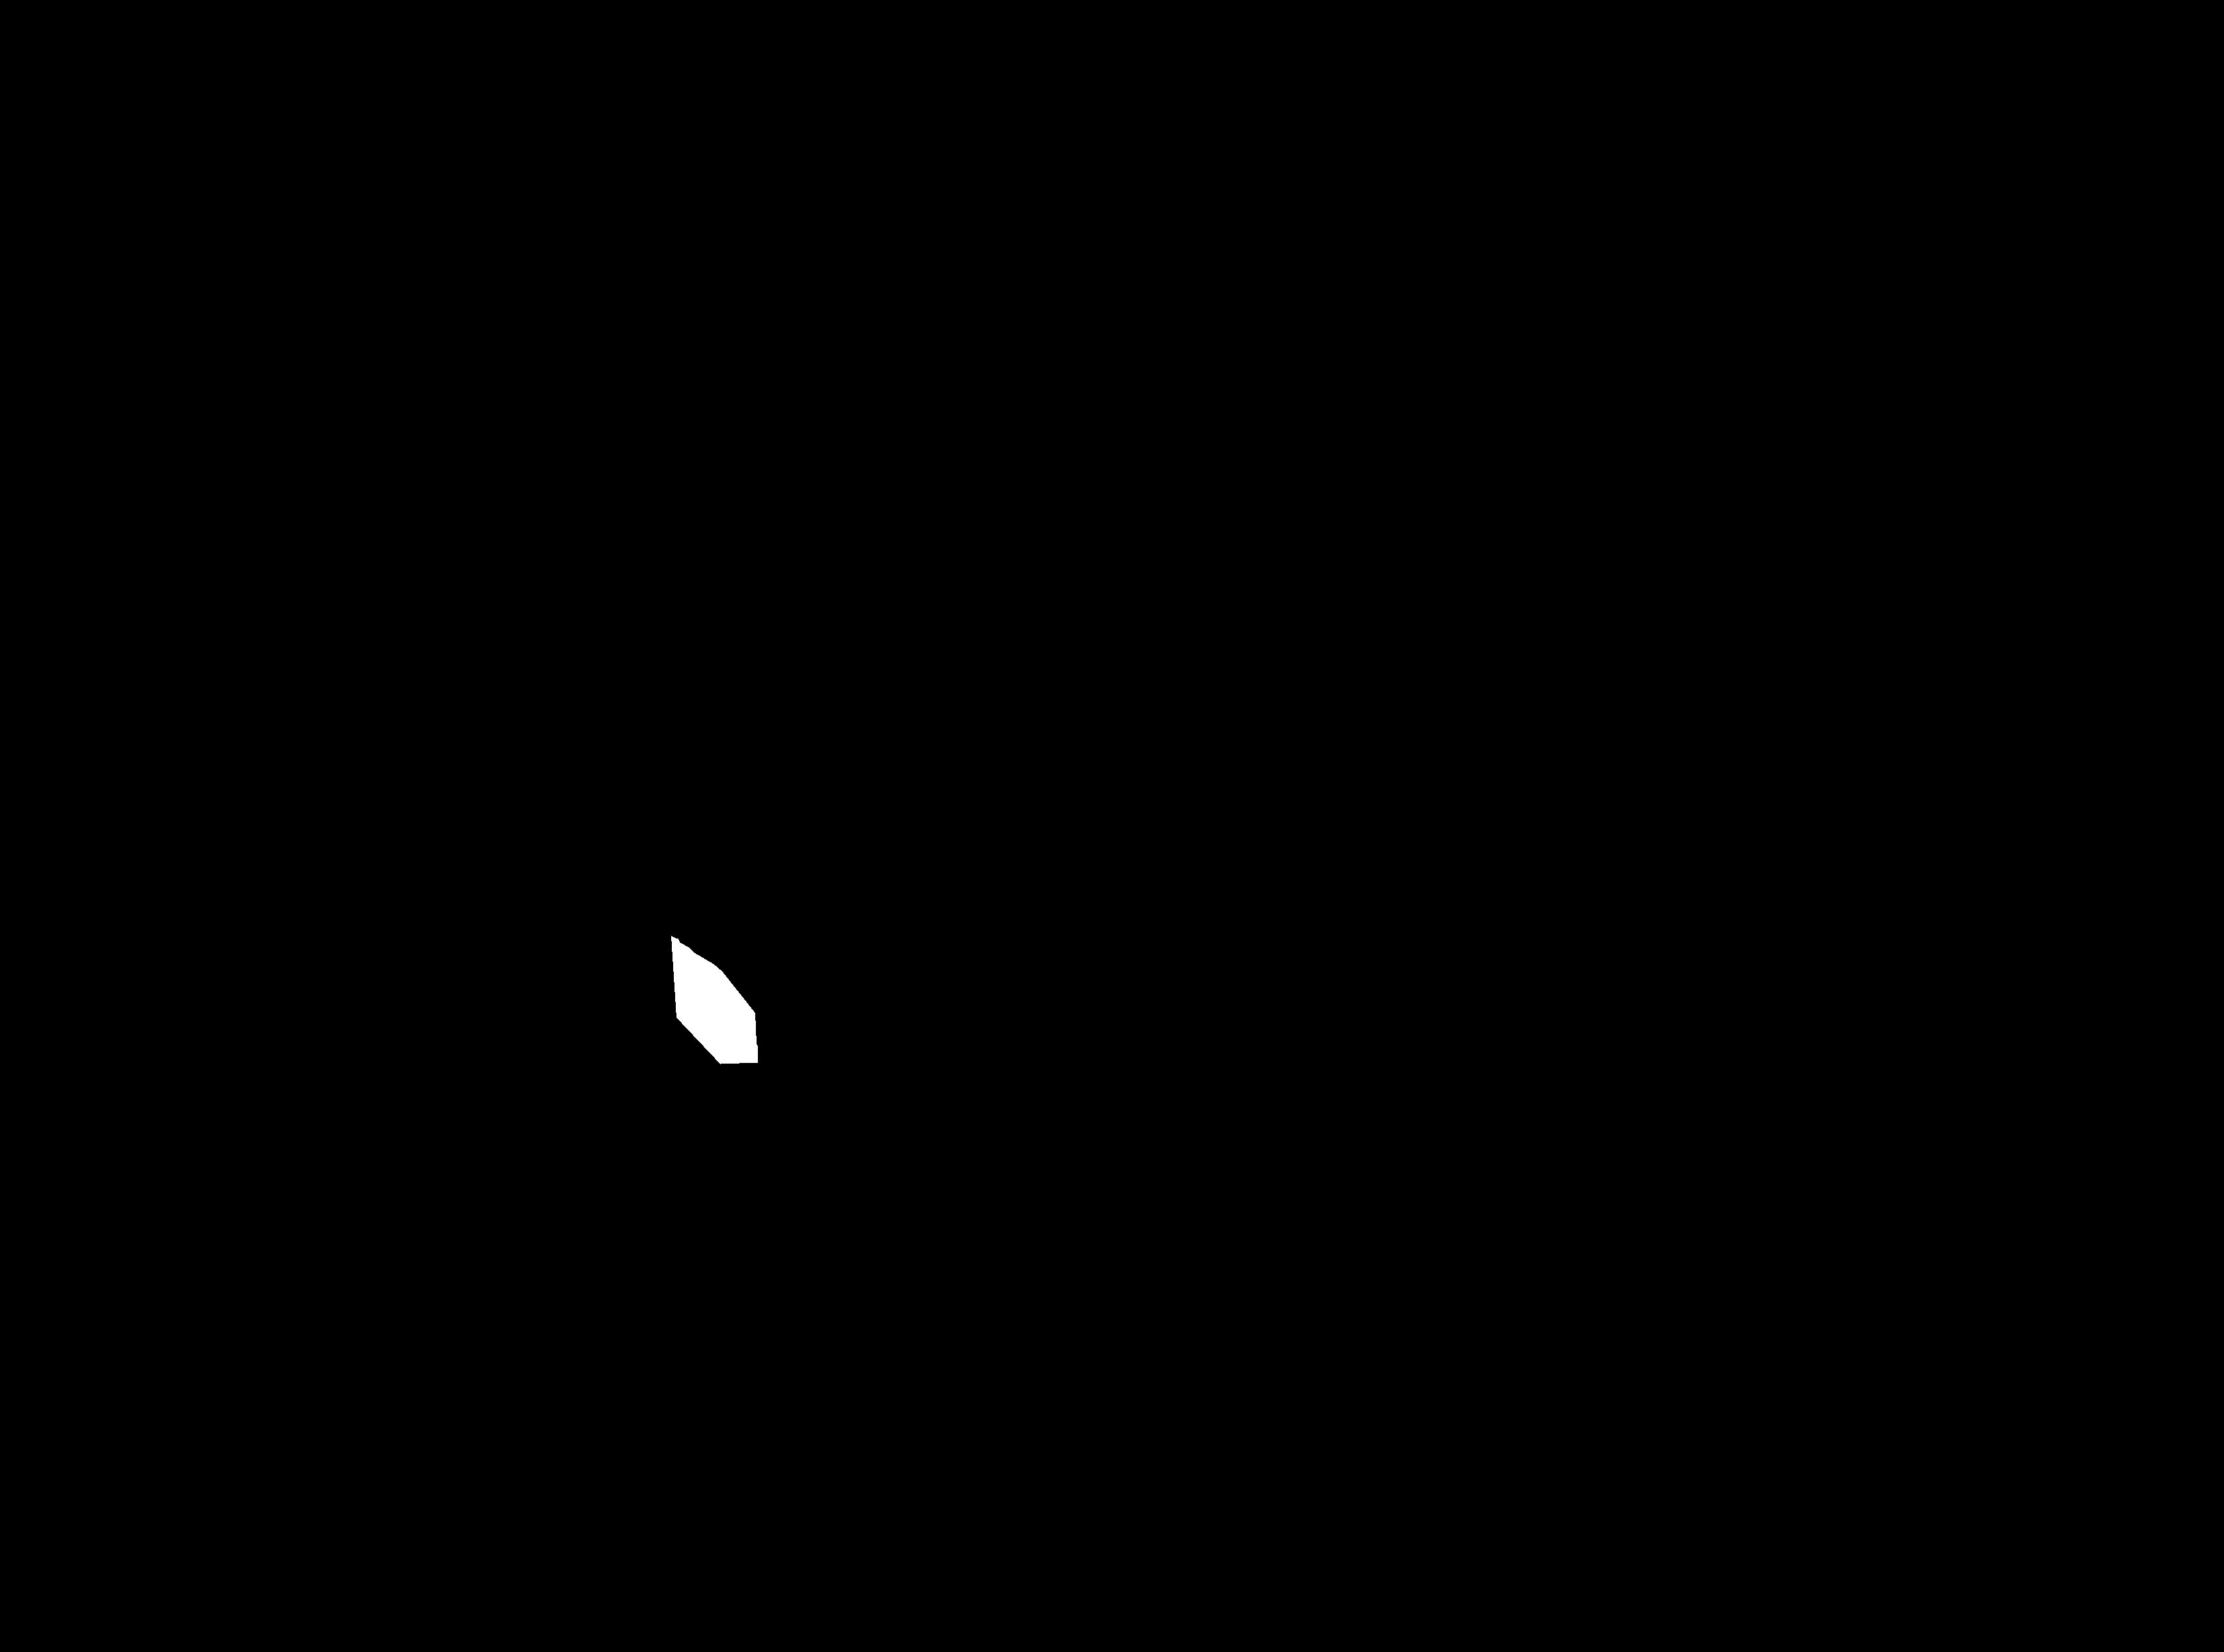
\includegraphics[width=0.475\textwidth]{figures/flatconnectordatasetimages/cut_corner_mask.png}
        \caption*{Cut Corner}

    \end{subfigure}
    \hfill
    \begin{subfigure}[b]{0.3\textwidth}
        \centering
        \includegraphics[width=0.475\textwidth]{figures/flatconnectordatasetimages/damaged_edge.png}
        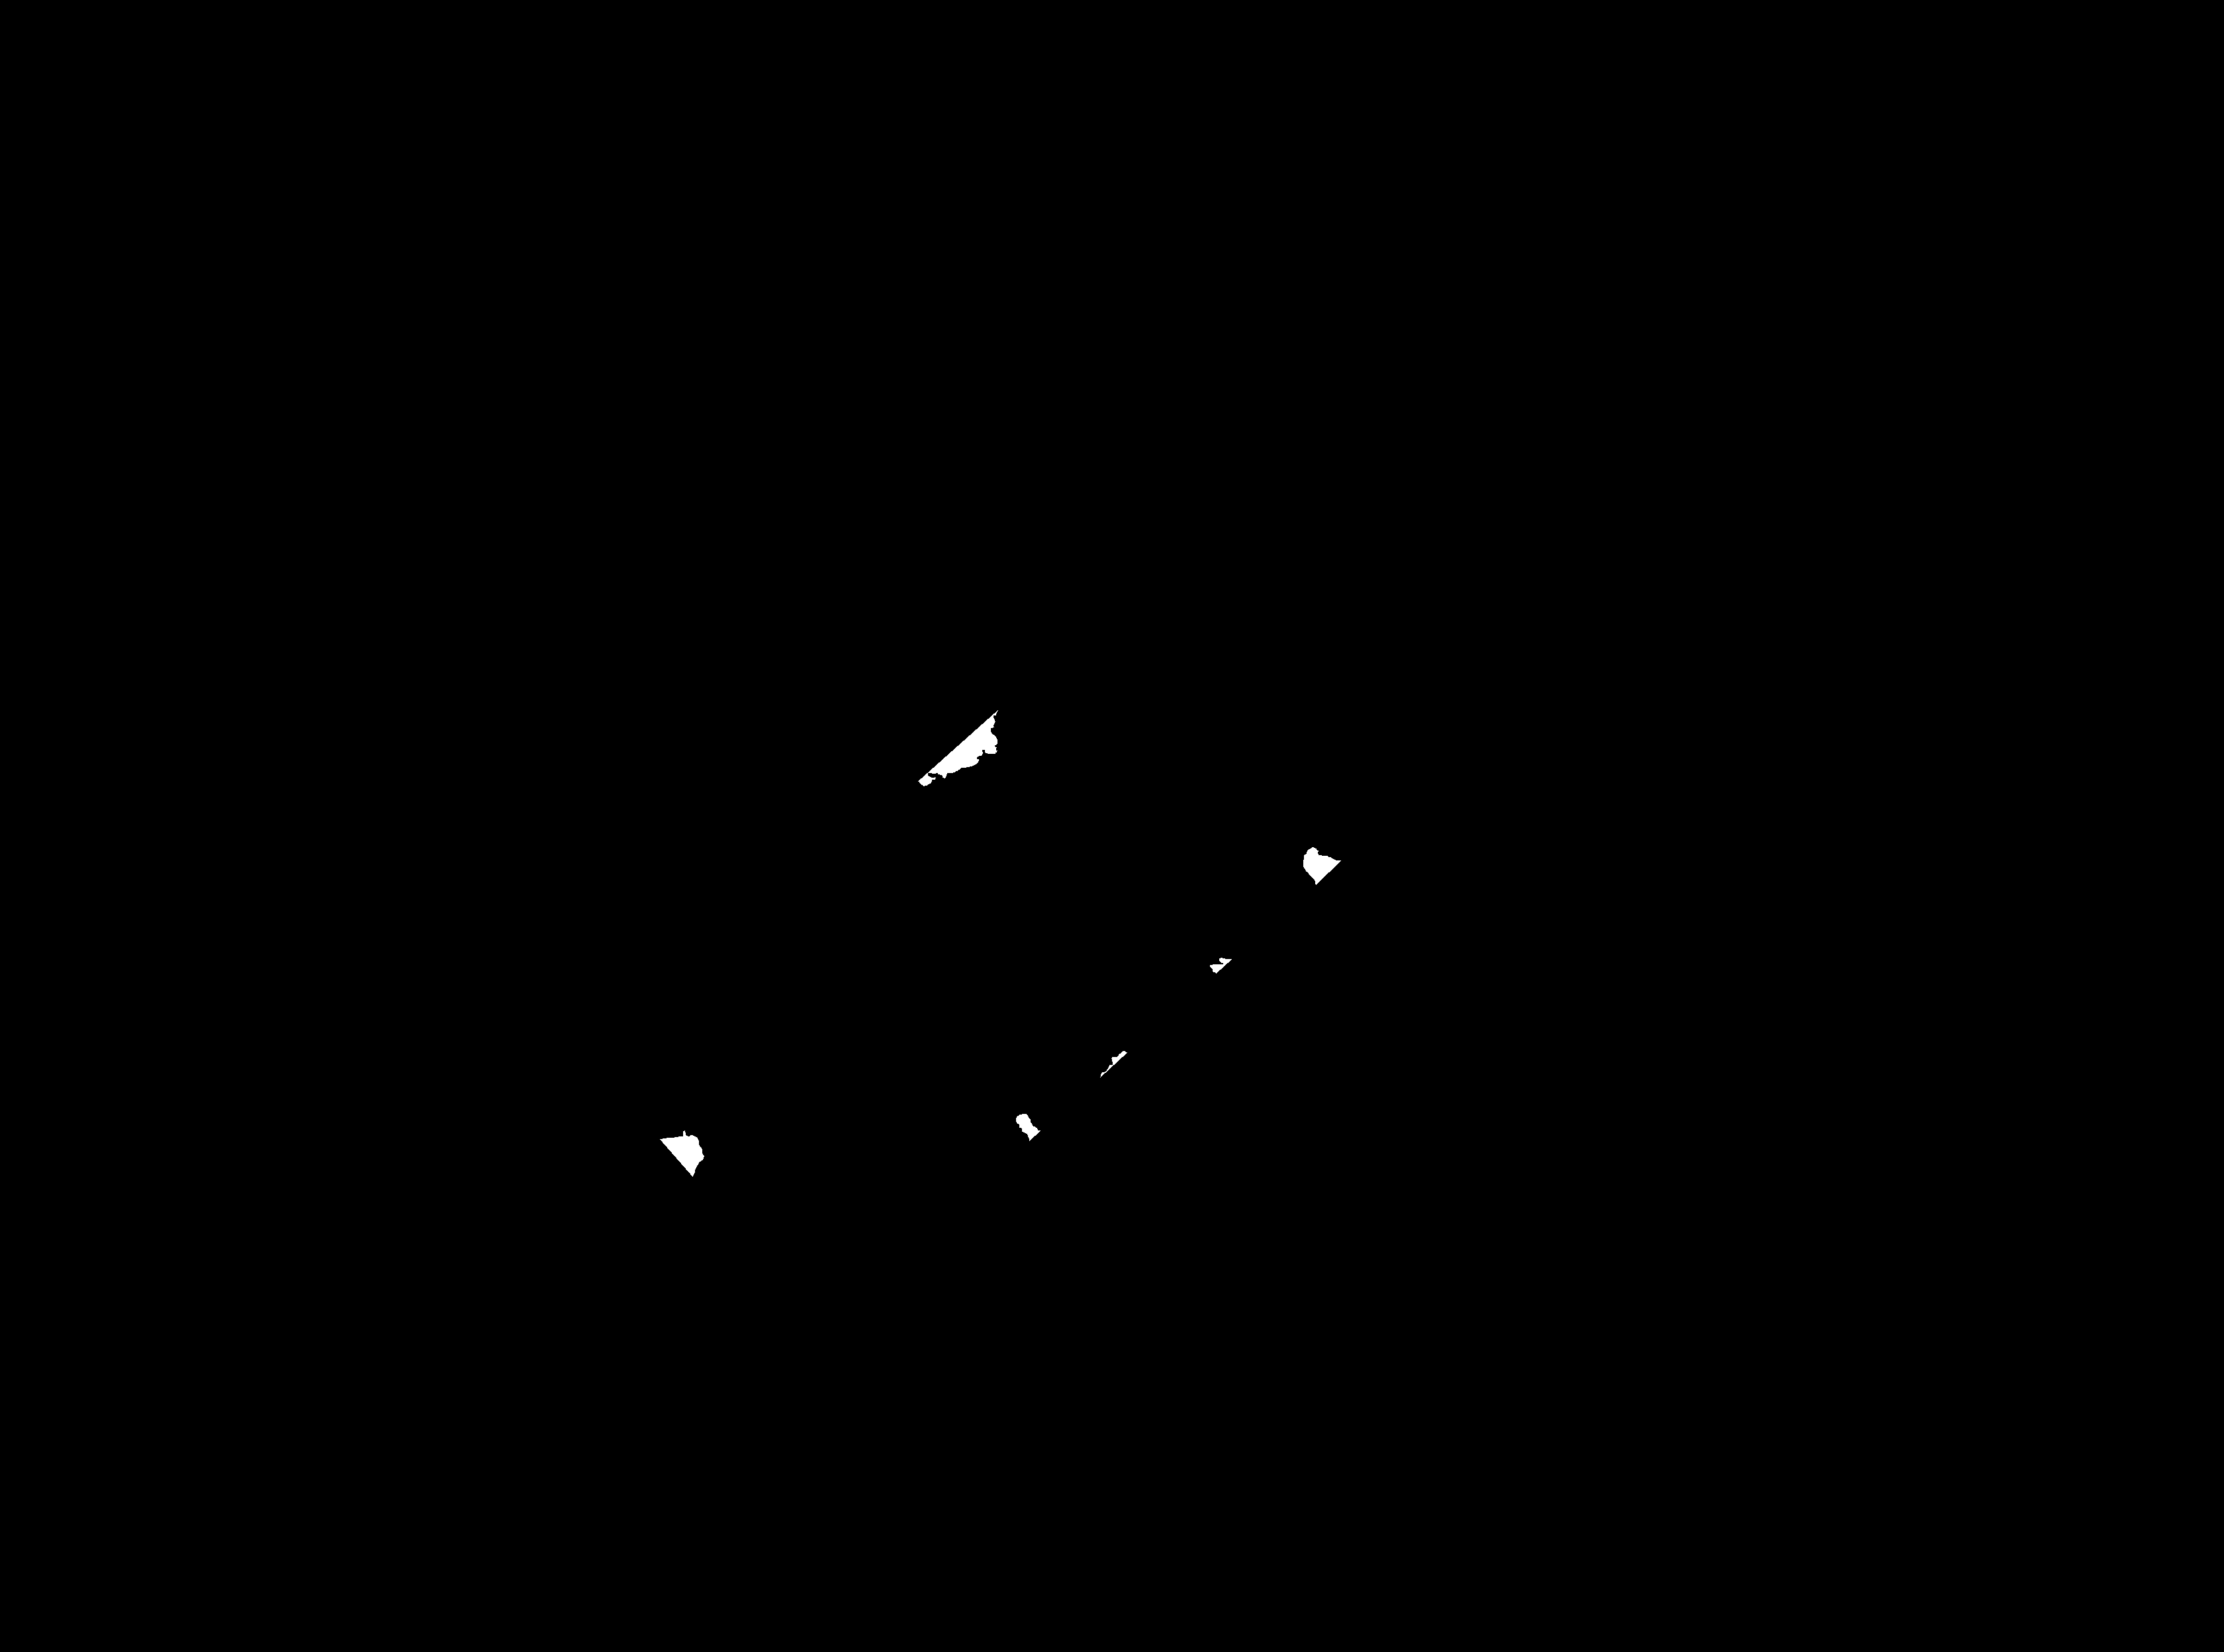
\includegraphics[width=0.475\textwidth]{figures/flatconnectordatasetimages/damaged_edge_mask.png}
        \caption*{Damaged Edge}

    \end{subfigure}
    \hfill
    \begin{subfigure}[b]{0.3\textwidth}
        \centering
        \includegraphics[width=0.475\textwidth]{figures/flatconnectordatasetimages/scratch.png}
        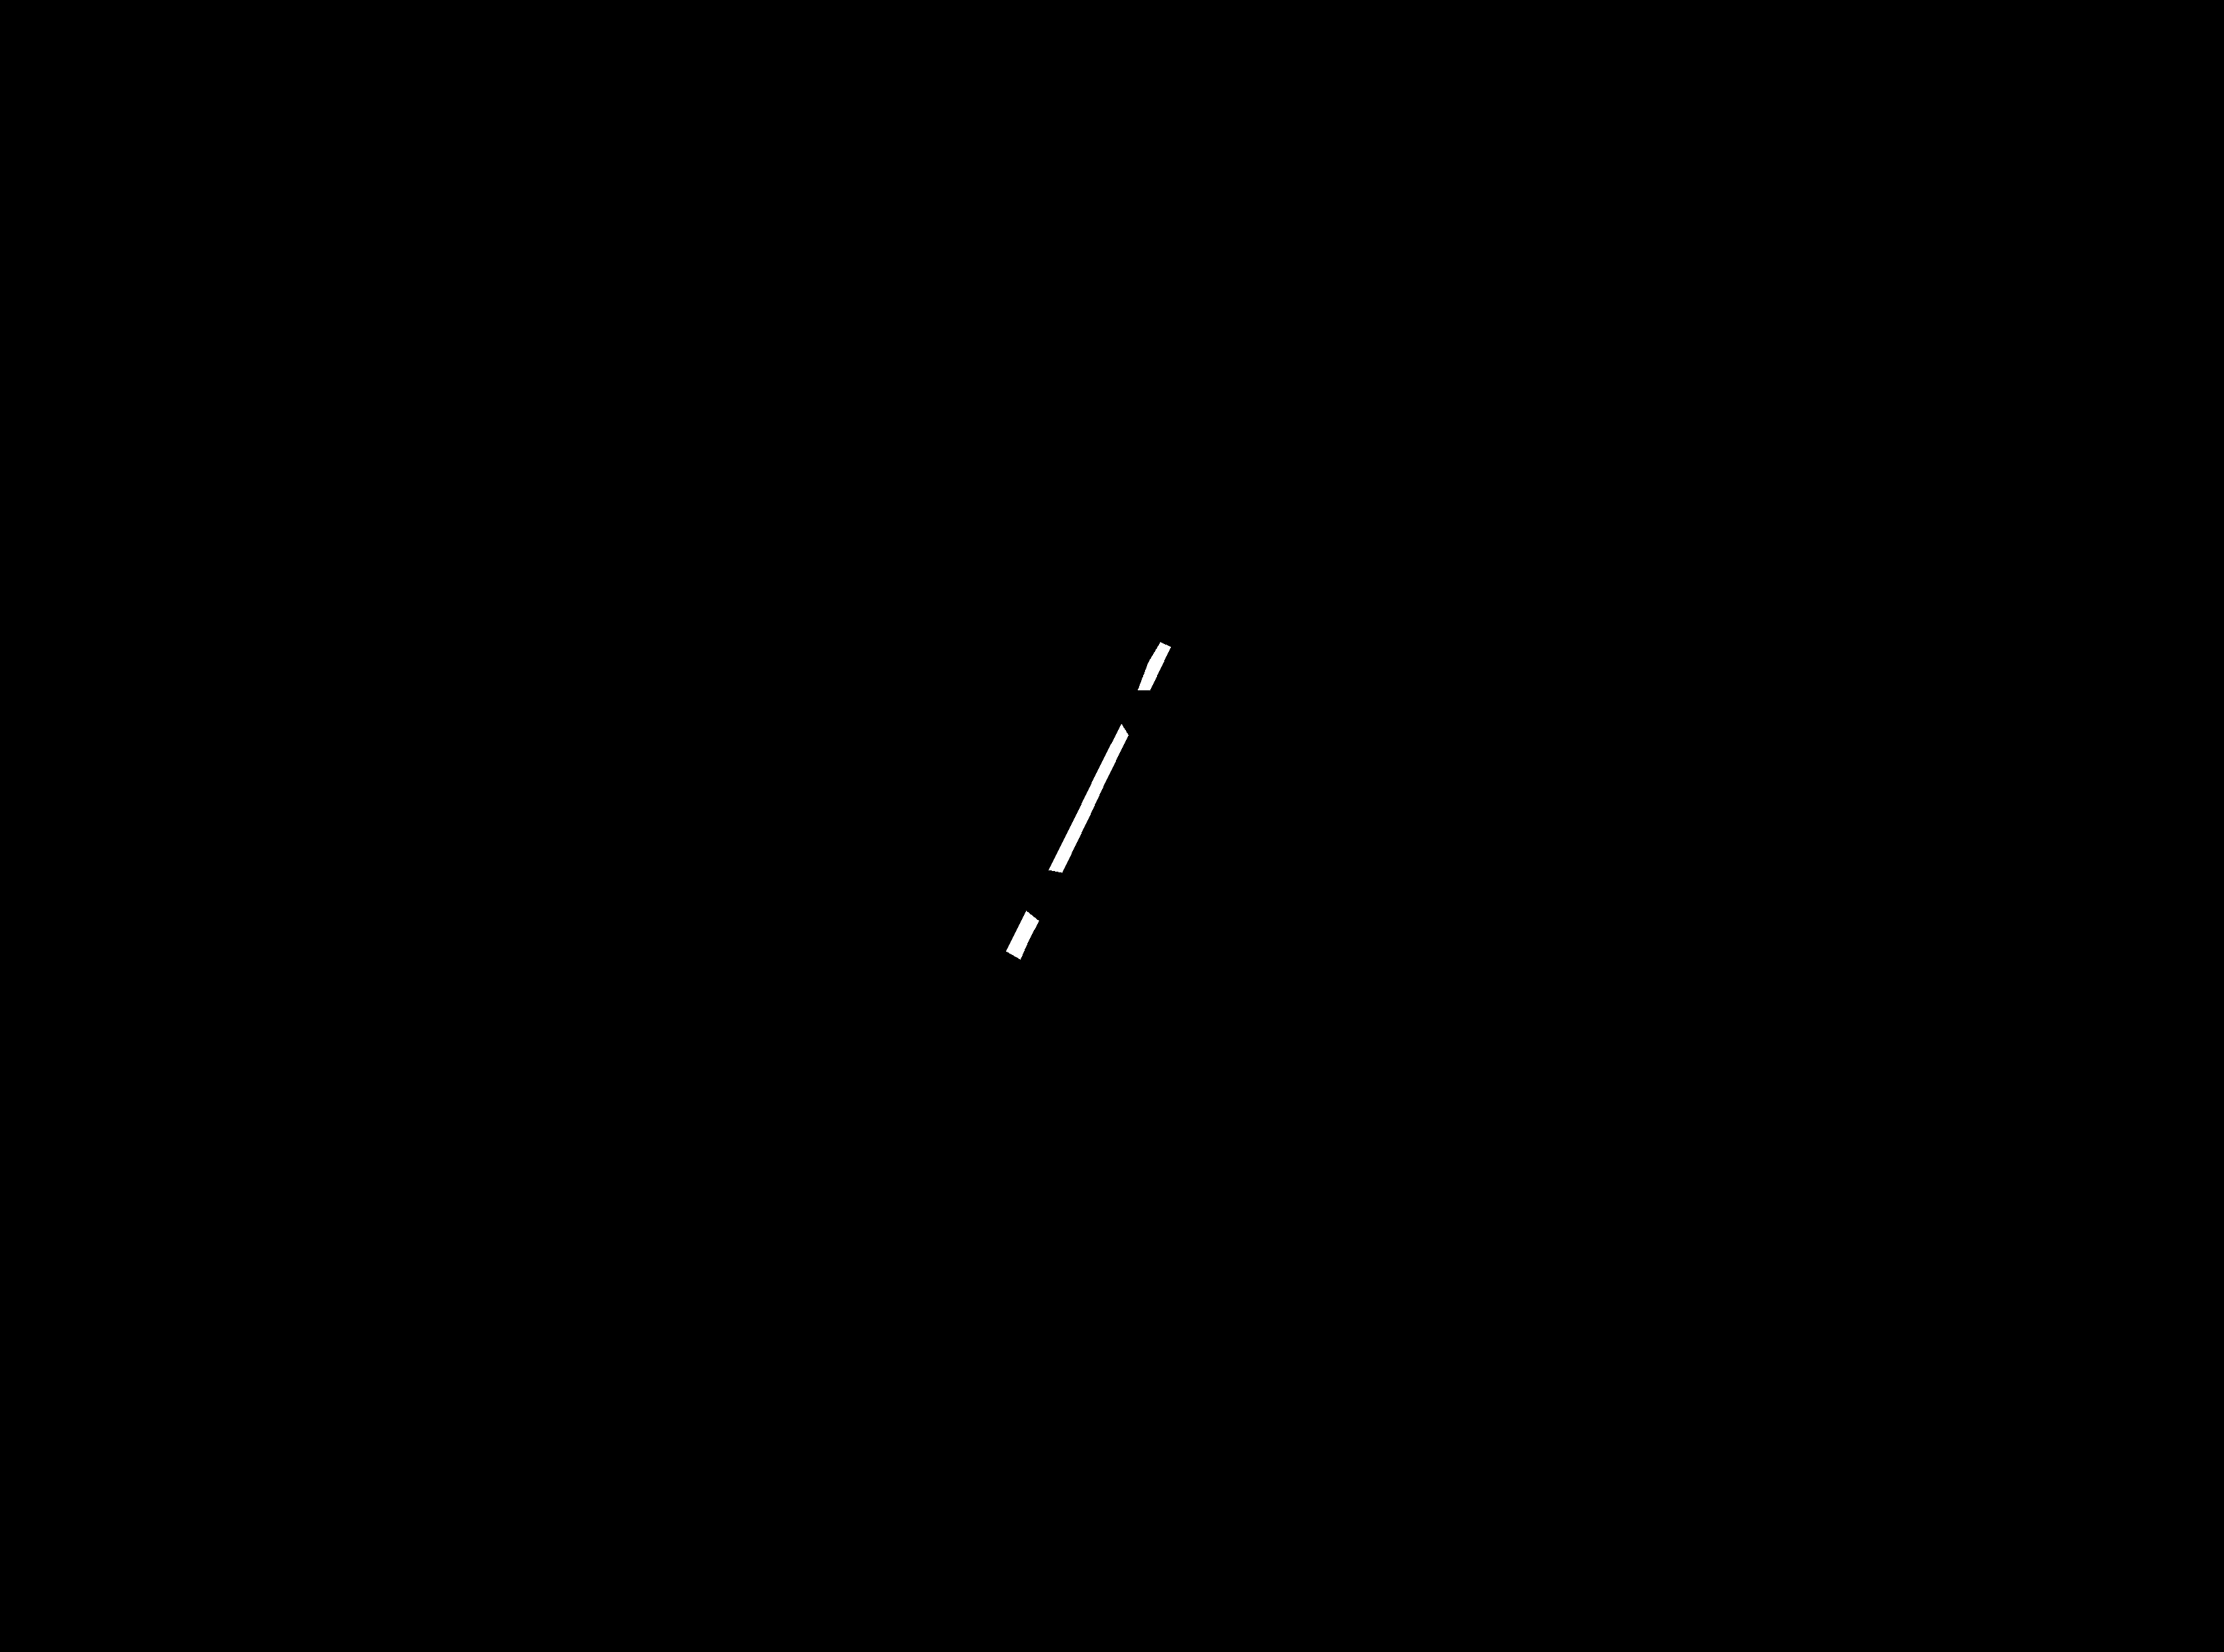
\includegraphics[width=0.475\textwidth]{figures/flatconnectordatasetimages/scratch_mask.png}
        \caption*{Scratch}

    \end{subfigure}
    \\
    \begin{subfigure}[b]{0.3\textwidth}
        \centering
        \includegraphics[width=0.475\textwidth]{figures/flatconnectordatasetimages/missing_big_hole.png}
        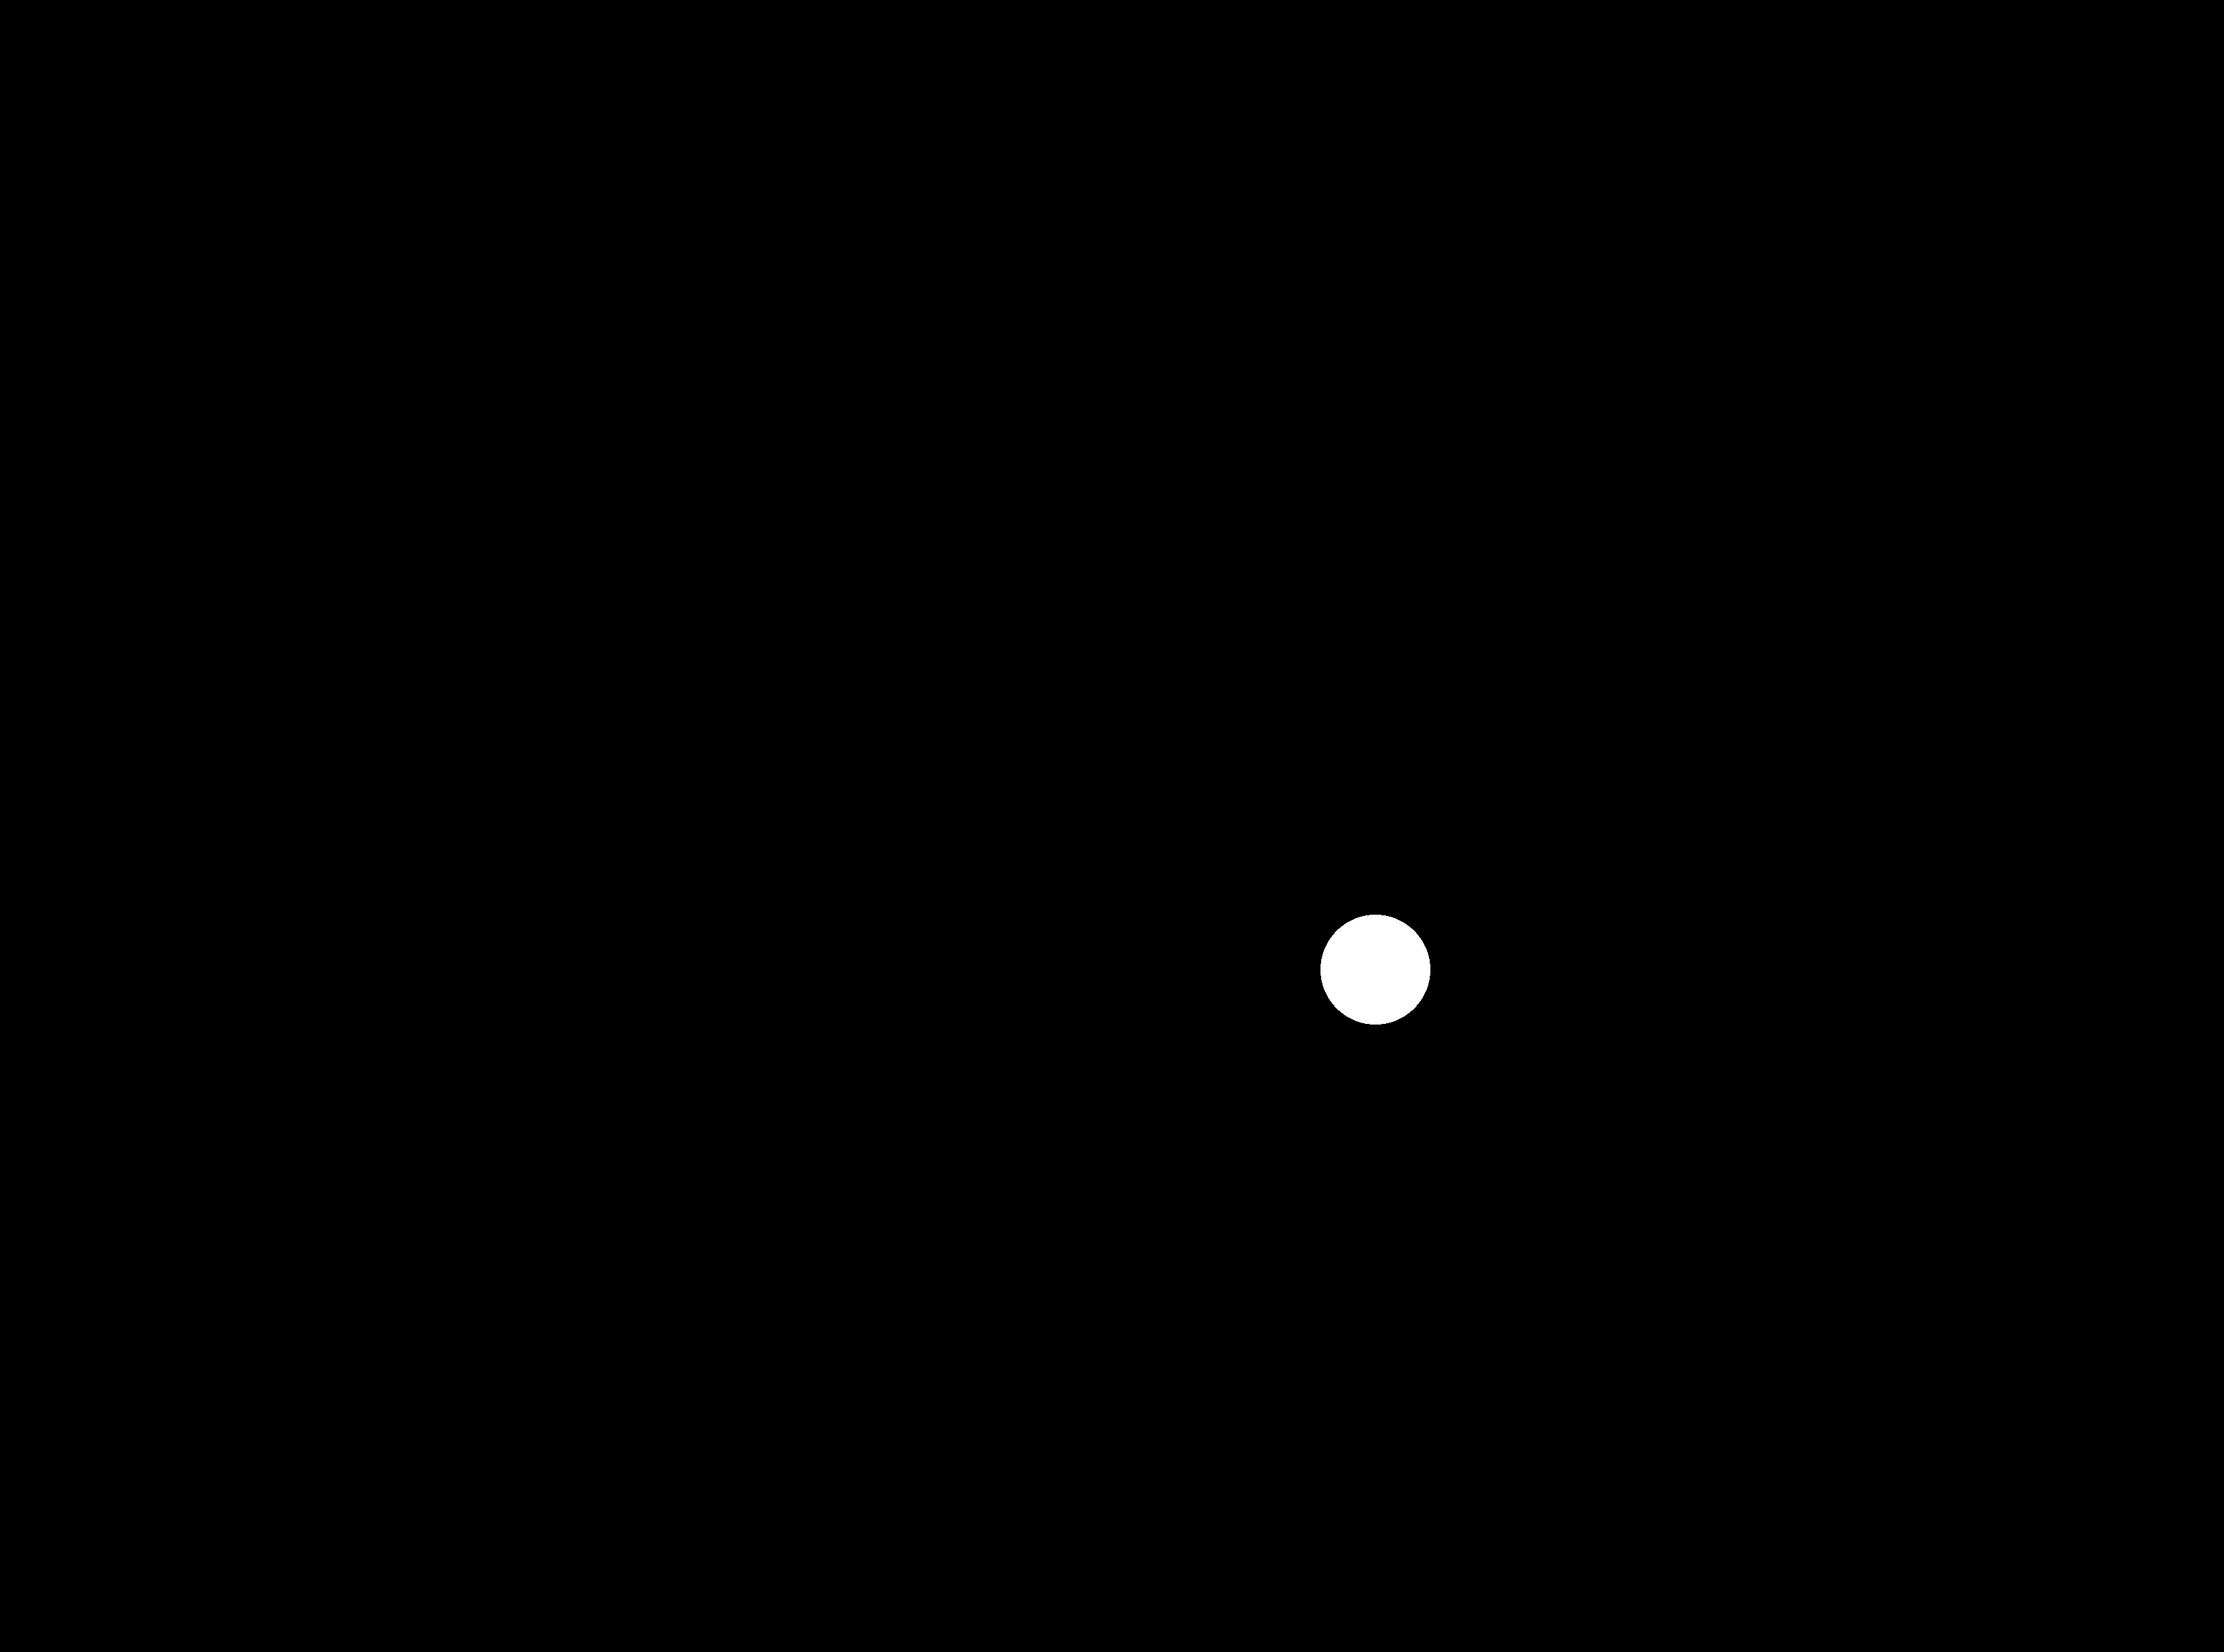
\includegraphics[width=0.475\textwidth]{figures/flatconnectordatasetimages/missing_big_hole_mask.png}
        \caption*{Missing Big Hole}

    \end{subfigure}
    \hfill
    \begin{subfigure}[b]{0.3\textwidth}
        \centering
        \includegraphics[width=0.475\textwidth]{figures/flatconnectordatasetimages/extra_holes.png}
        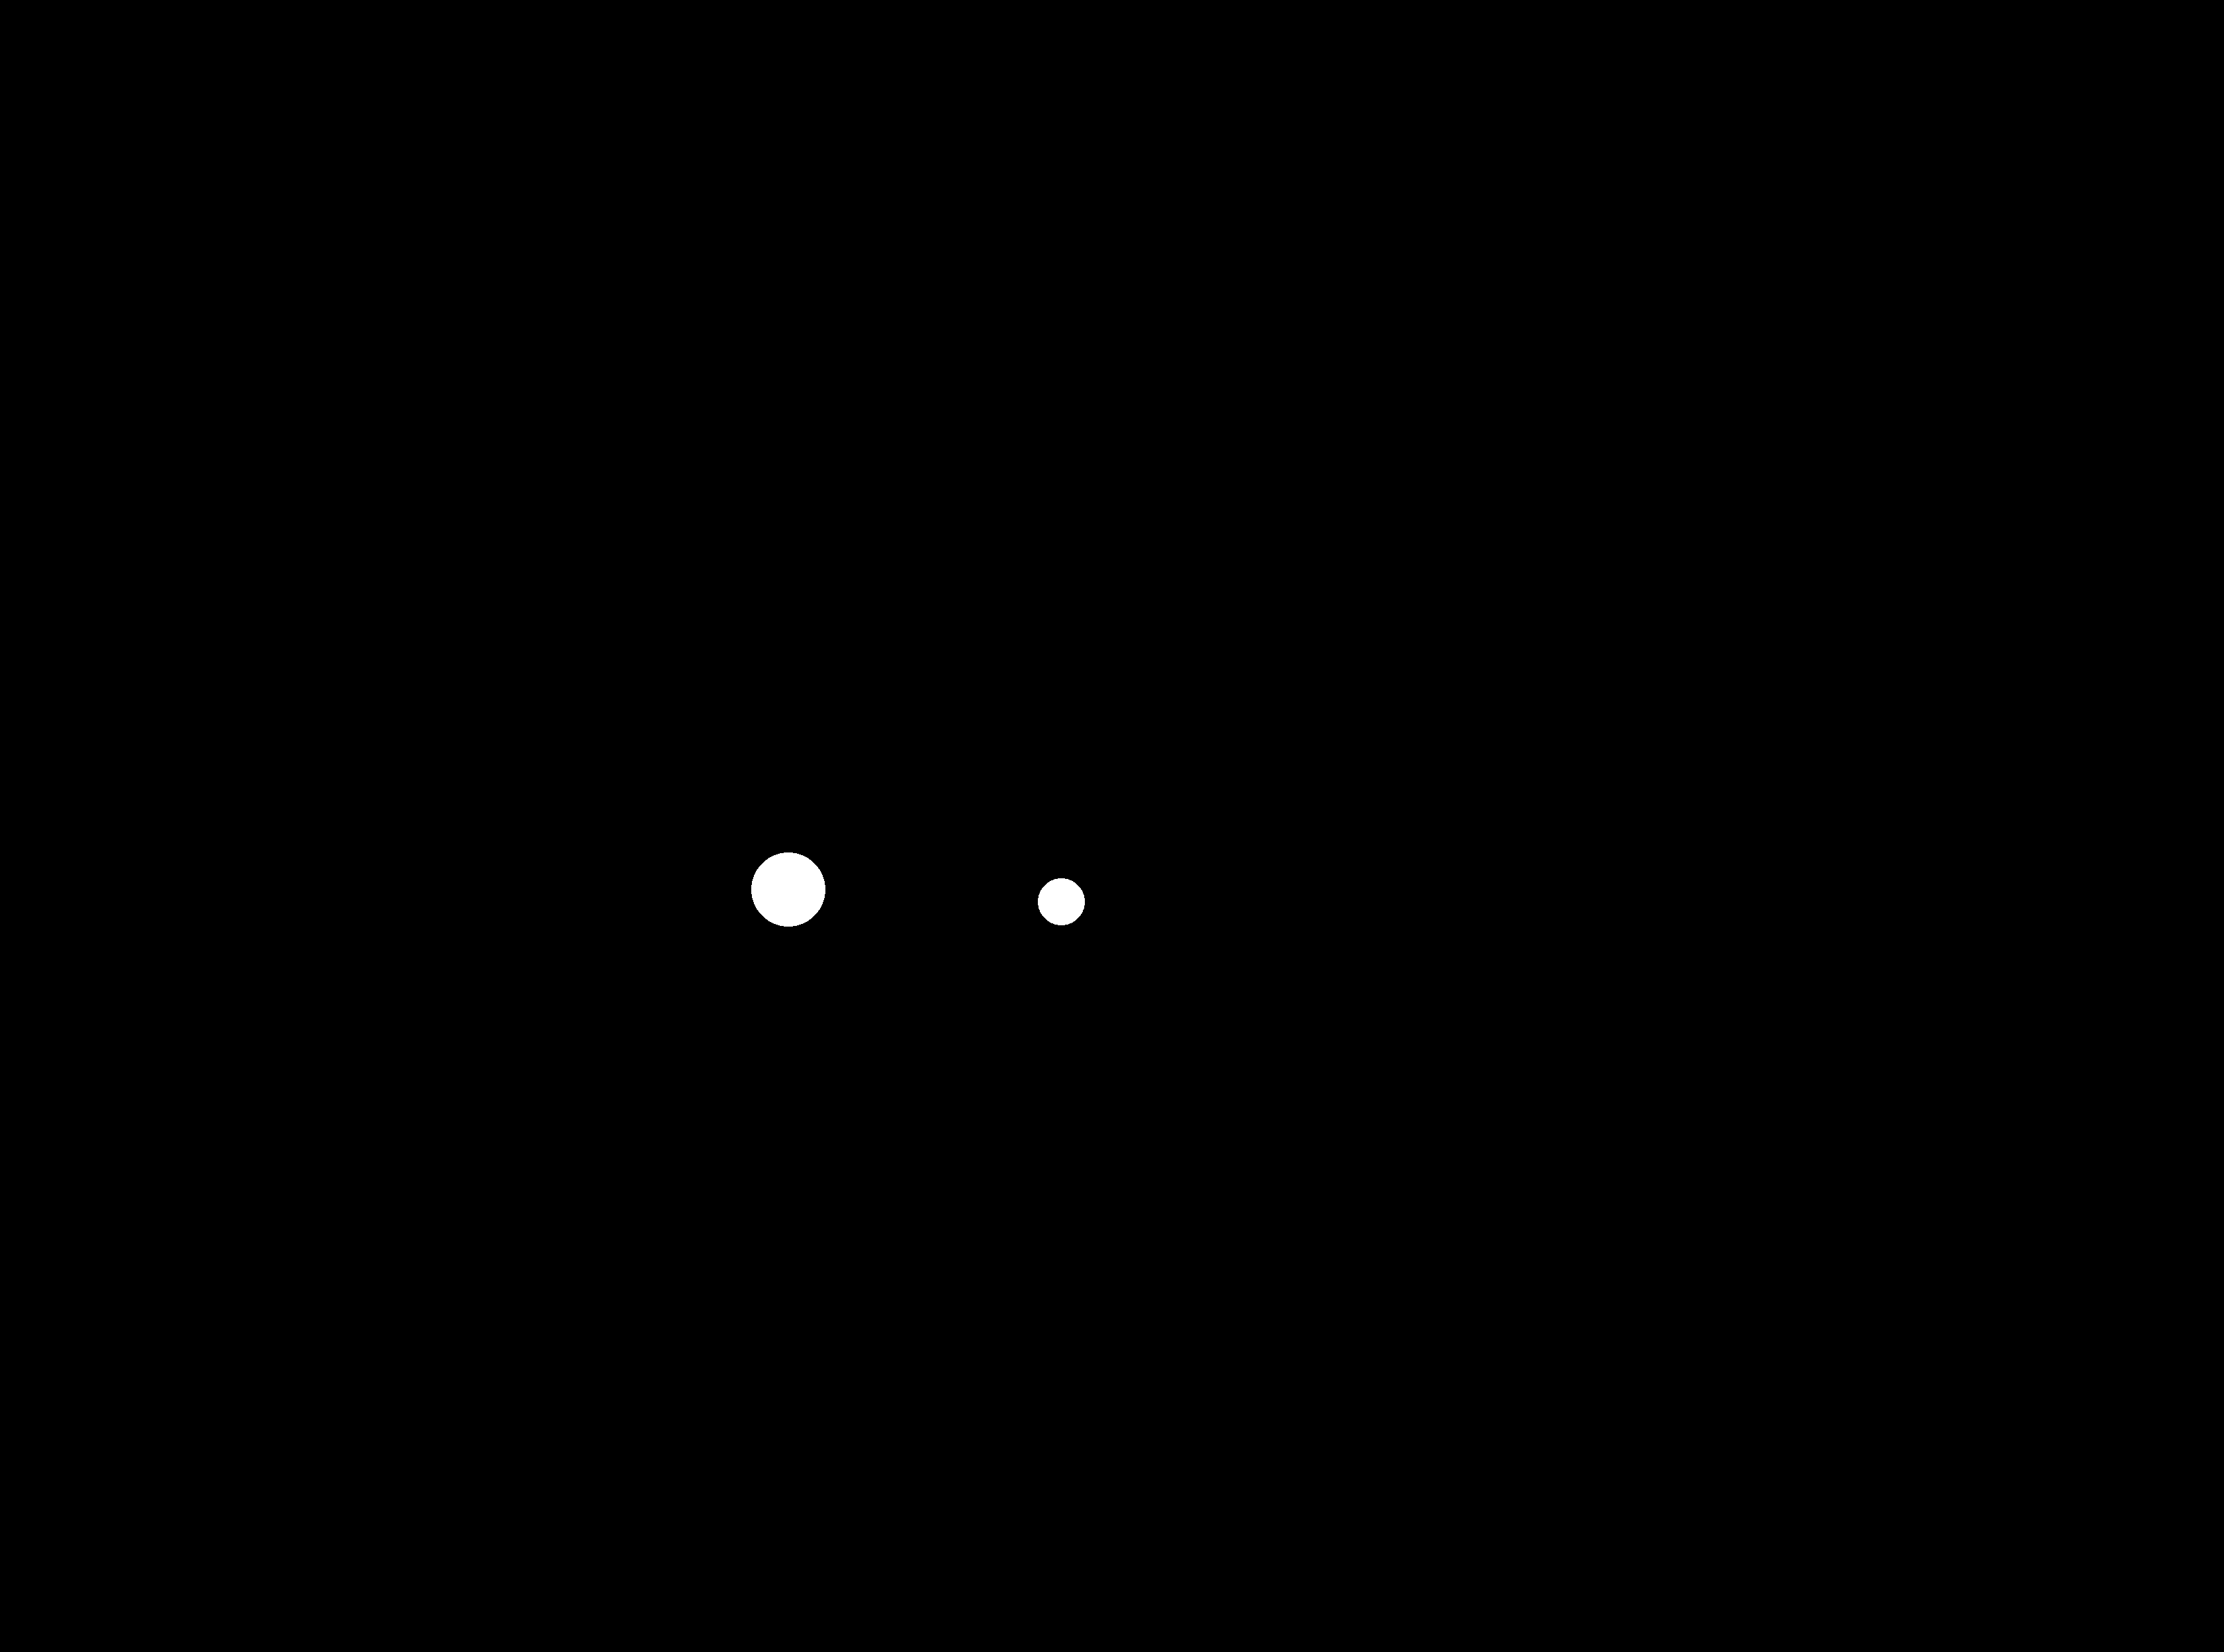
\includegraphics[width=0.475\textwidth]{figures/flatconnectordatasetimages/extra_holes_mask.png}
        \caption*{Extra Holes}

    \end{subfigure}
    \hfill
    \begin{subfigure}[b]{0.3\textwidth}
        \centering
        \includegraphics[width=0.475\textwidth]{figures/flatconnectordatasetimages/diff_size_holes.png}
        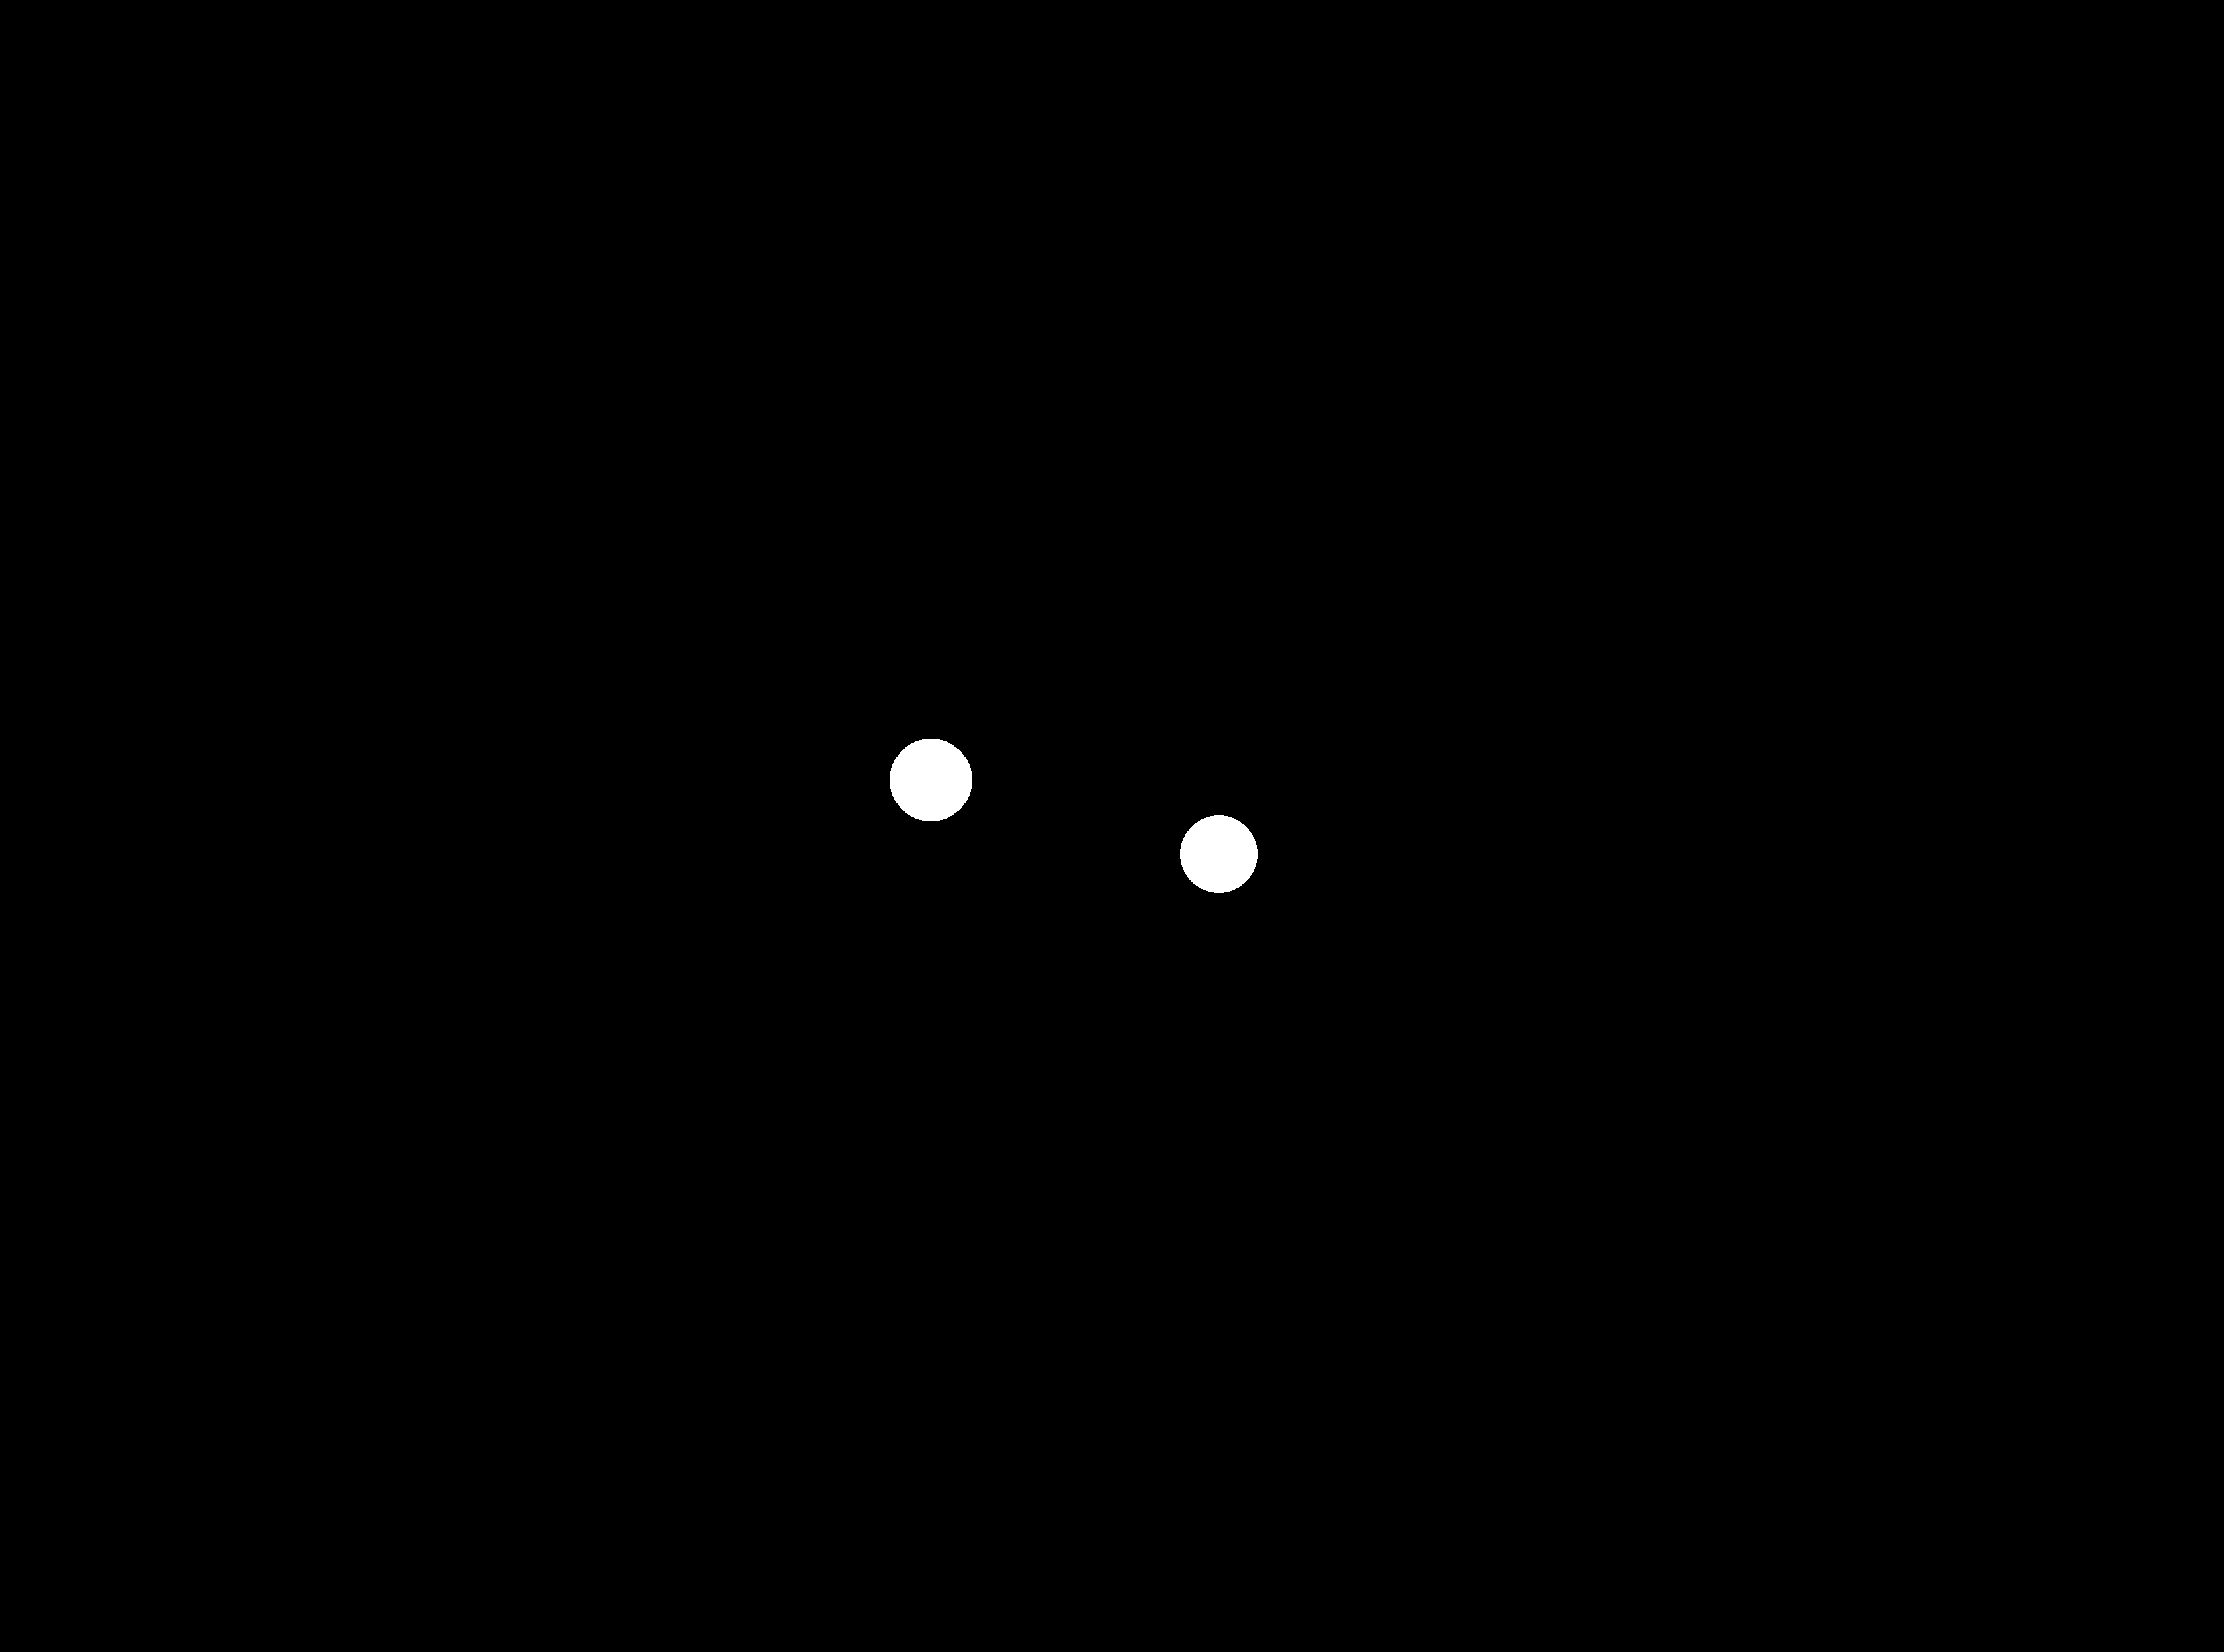
\includegraphics[width=0.475\textwidth]{figures/flatconnectordatasetimages/diff_size_holes_mask.png}
        \caption*{Differently Sized Holes}

    \end{subfigure}
    %\captionsetup{justification=centering, skip=-10pt}
    \caption{Anomalous Flat Connector Images and the Corresponding Masks}
    \label{fig:flatconnectorexampleimages}
\end{figure}






\section{Data Acquisition Setup}
\label{sec:faltconnectordataacquisiton}

The images for the dataset were taken in the university facilities. An exemplary setup for image acquisition can be viewed in figure xyz(images von setup). The contraption to capture images was 
done by mounting a camera on to a pole that was attached to a small table, pointing the camera lens at the table from an overhead perspective. The distance between camera lens and the table surface was approximately (angabe) cm and the main light source in the 
images was delivered by a softbox(stimmt das?). Regarding the background of the object, a black cloth was chosen to be layed flat on the table, where the object would then be put. For 
an increased variety, multiple flat connectors were bought and filmed. Here each one was manually rotated after each shot, to acheive different object orientations and thus a more robust training 
set. Each flat connector was rotated a total of six times per side, resulting in 12 normal images per flat connector object. \newline
The camera used to take pictures was a (camera modell) which produced the images of the flat connectors in a (pixel angaben) resolution. (guccken obs stimmt) Due to the large size of the resulting 
images, they were resized to (pixel angaben) with amounts to roughly (prozen angabe) \% of the original image size.\newline
To obtain segmentation labels, a free polygon annotation software was used to then label anomalous regions in the images. The annotations were done by hand and by the author of this work. In accord to 
MVTecAD LOCO standards \cite{LOCODentsAndScratchesBergmann2022} each kind of anomaly would be assigned a different pixel value to differentiate them when working with saturation thresholds 
as mentioned in setion \ref{sec:datasets}. Example annotations can be viewed in figure xyz, where several original images are depicted next to the produced segmentation labels. Just like in the 
original MVTecAD LOCO dataset, image labels were not explicitly given since they can be inferred by the anomaly class.


\begin{figure}[htbp]
    \captionsetup[subfigure]{justification=centering}
    \centering
    \begin{subfigure}[b]{0.3\textwidth}
        \centering
        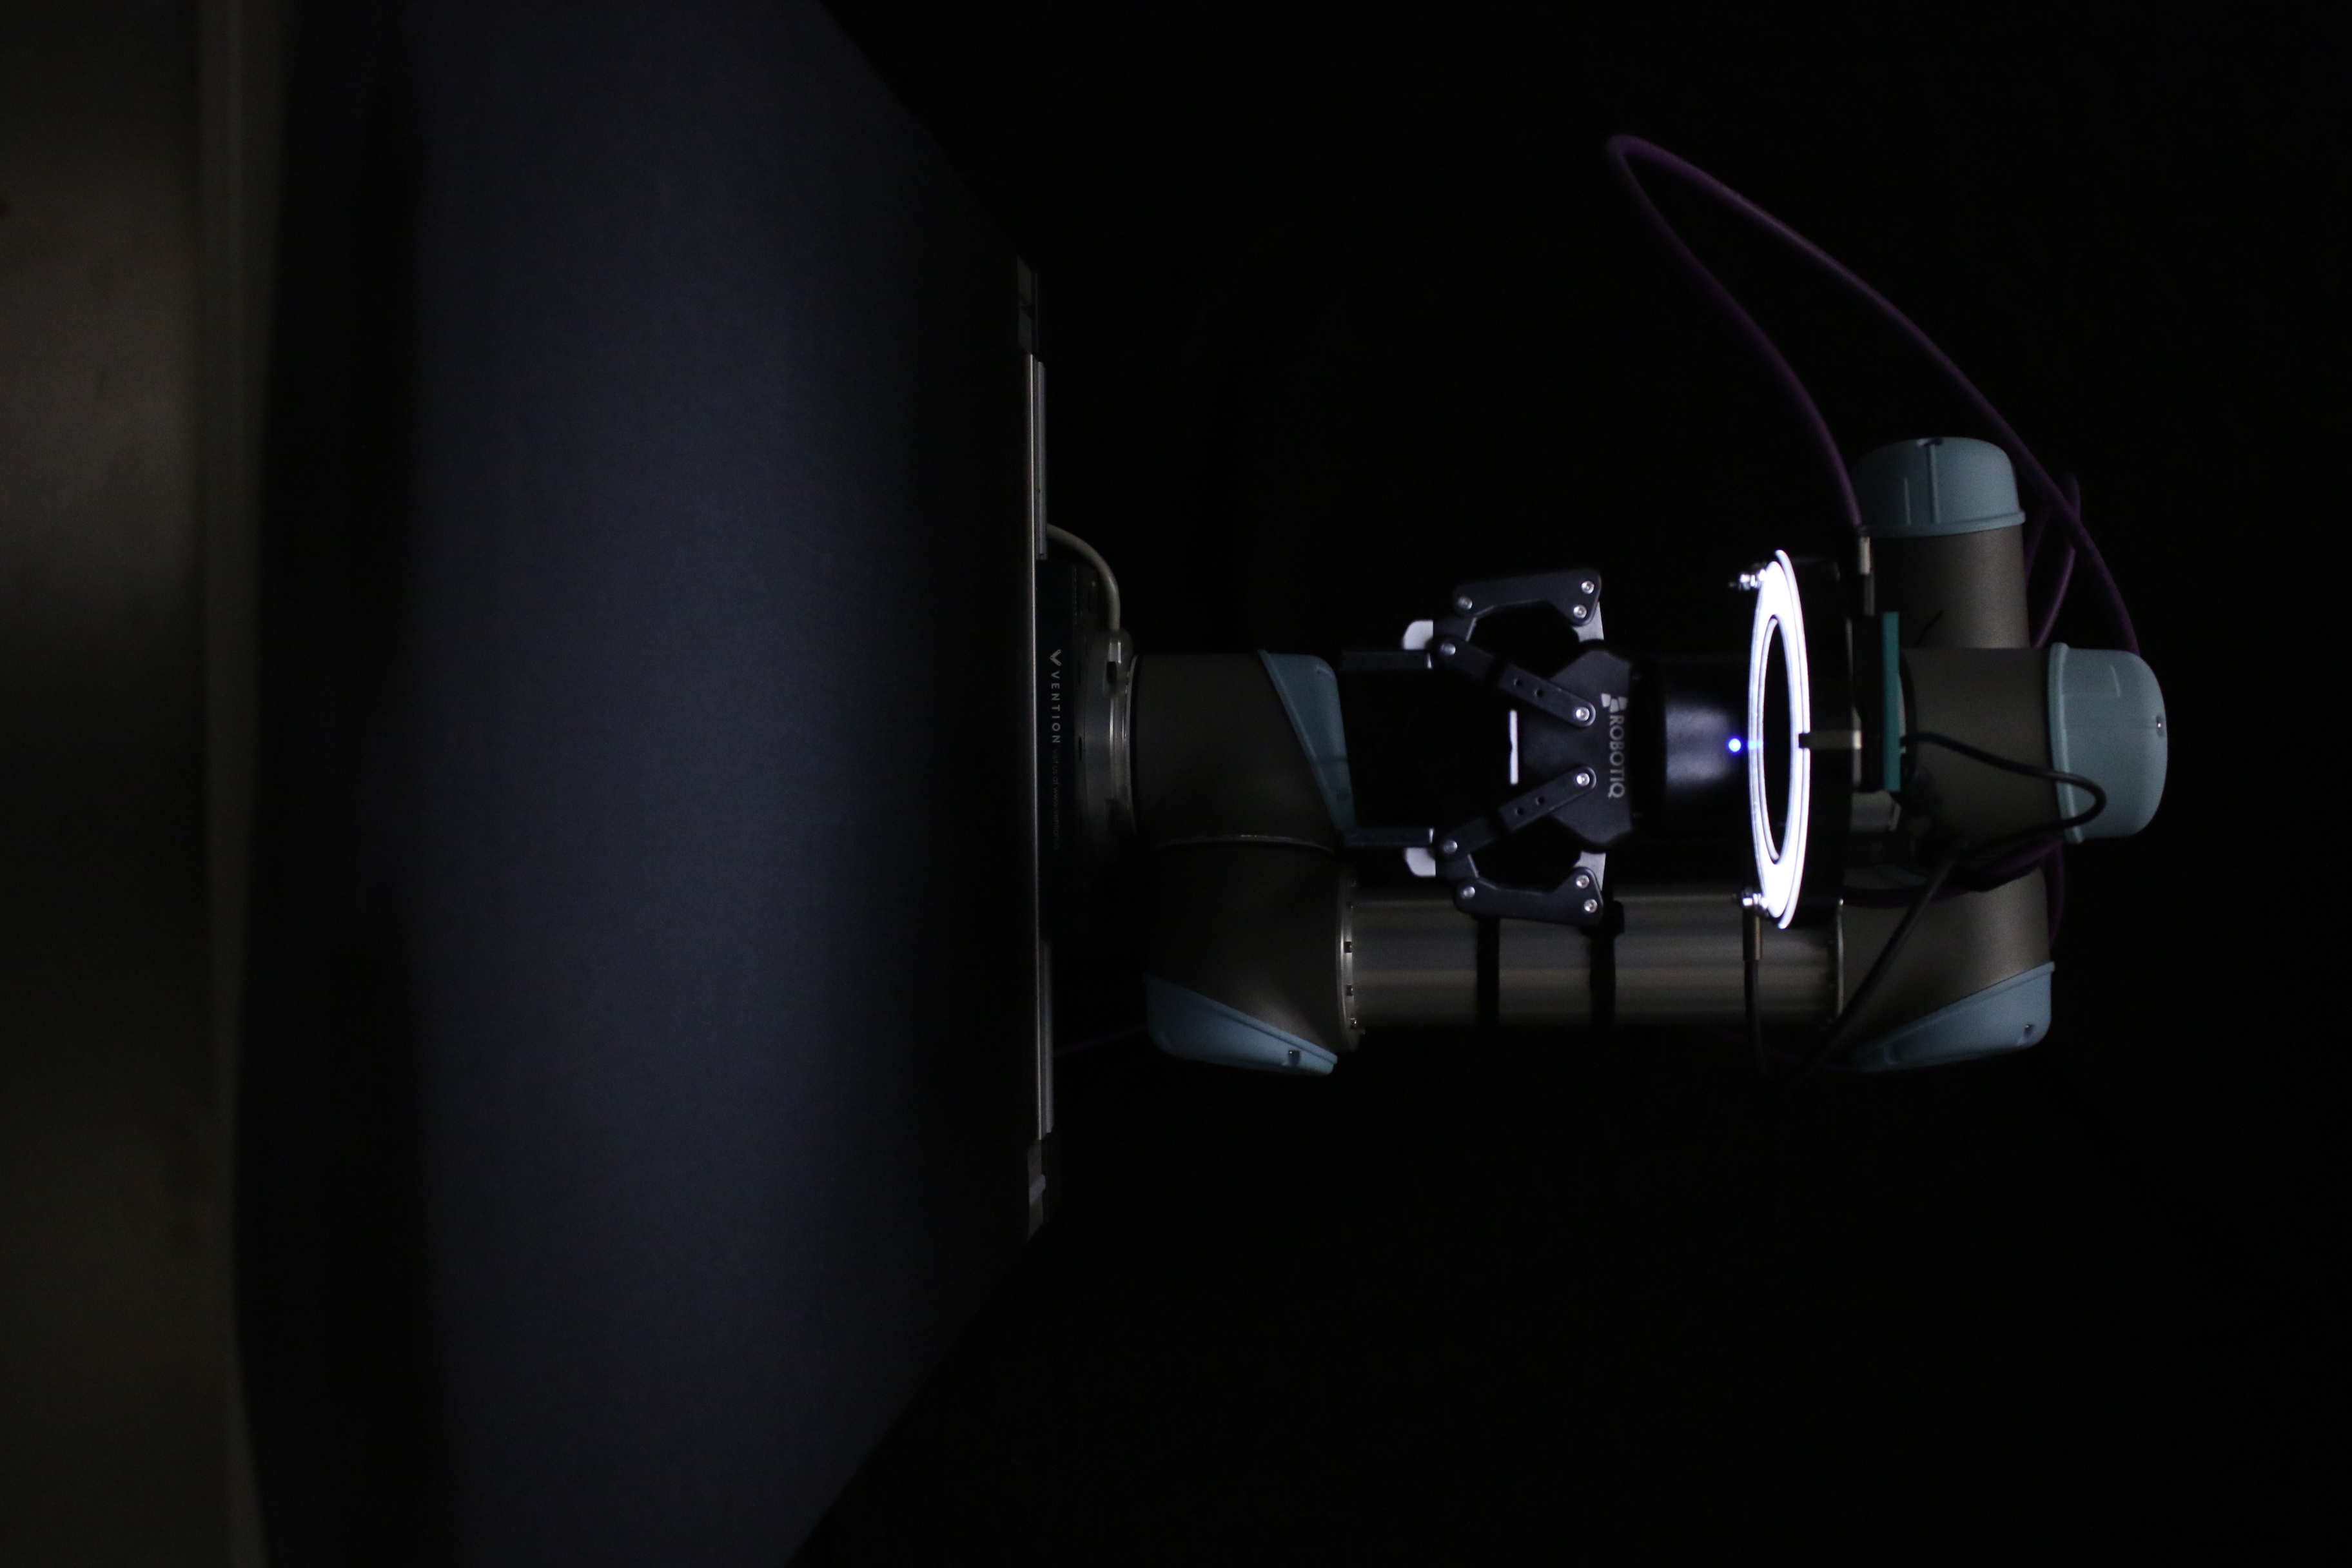
\includegraphics[angle=90, width=\textwidth]{figures/setupimages/setup_empty.JPG}


    \end{subfigure}
    \begin{subfigure}[b]{0.3\textwidth}
        \centering
        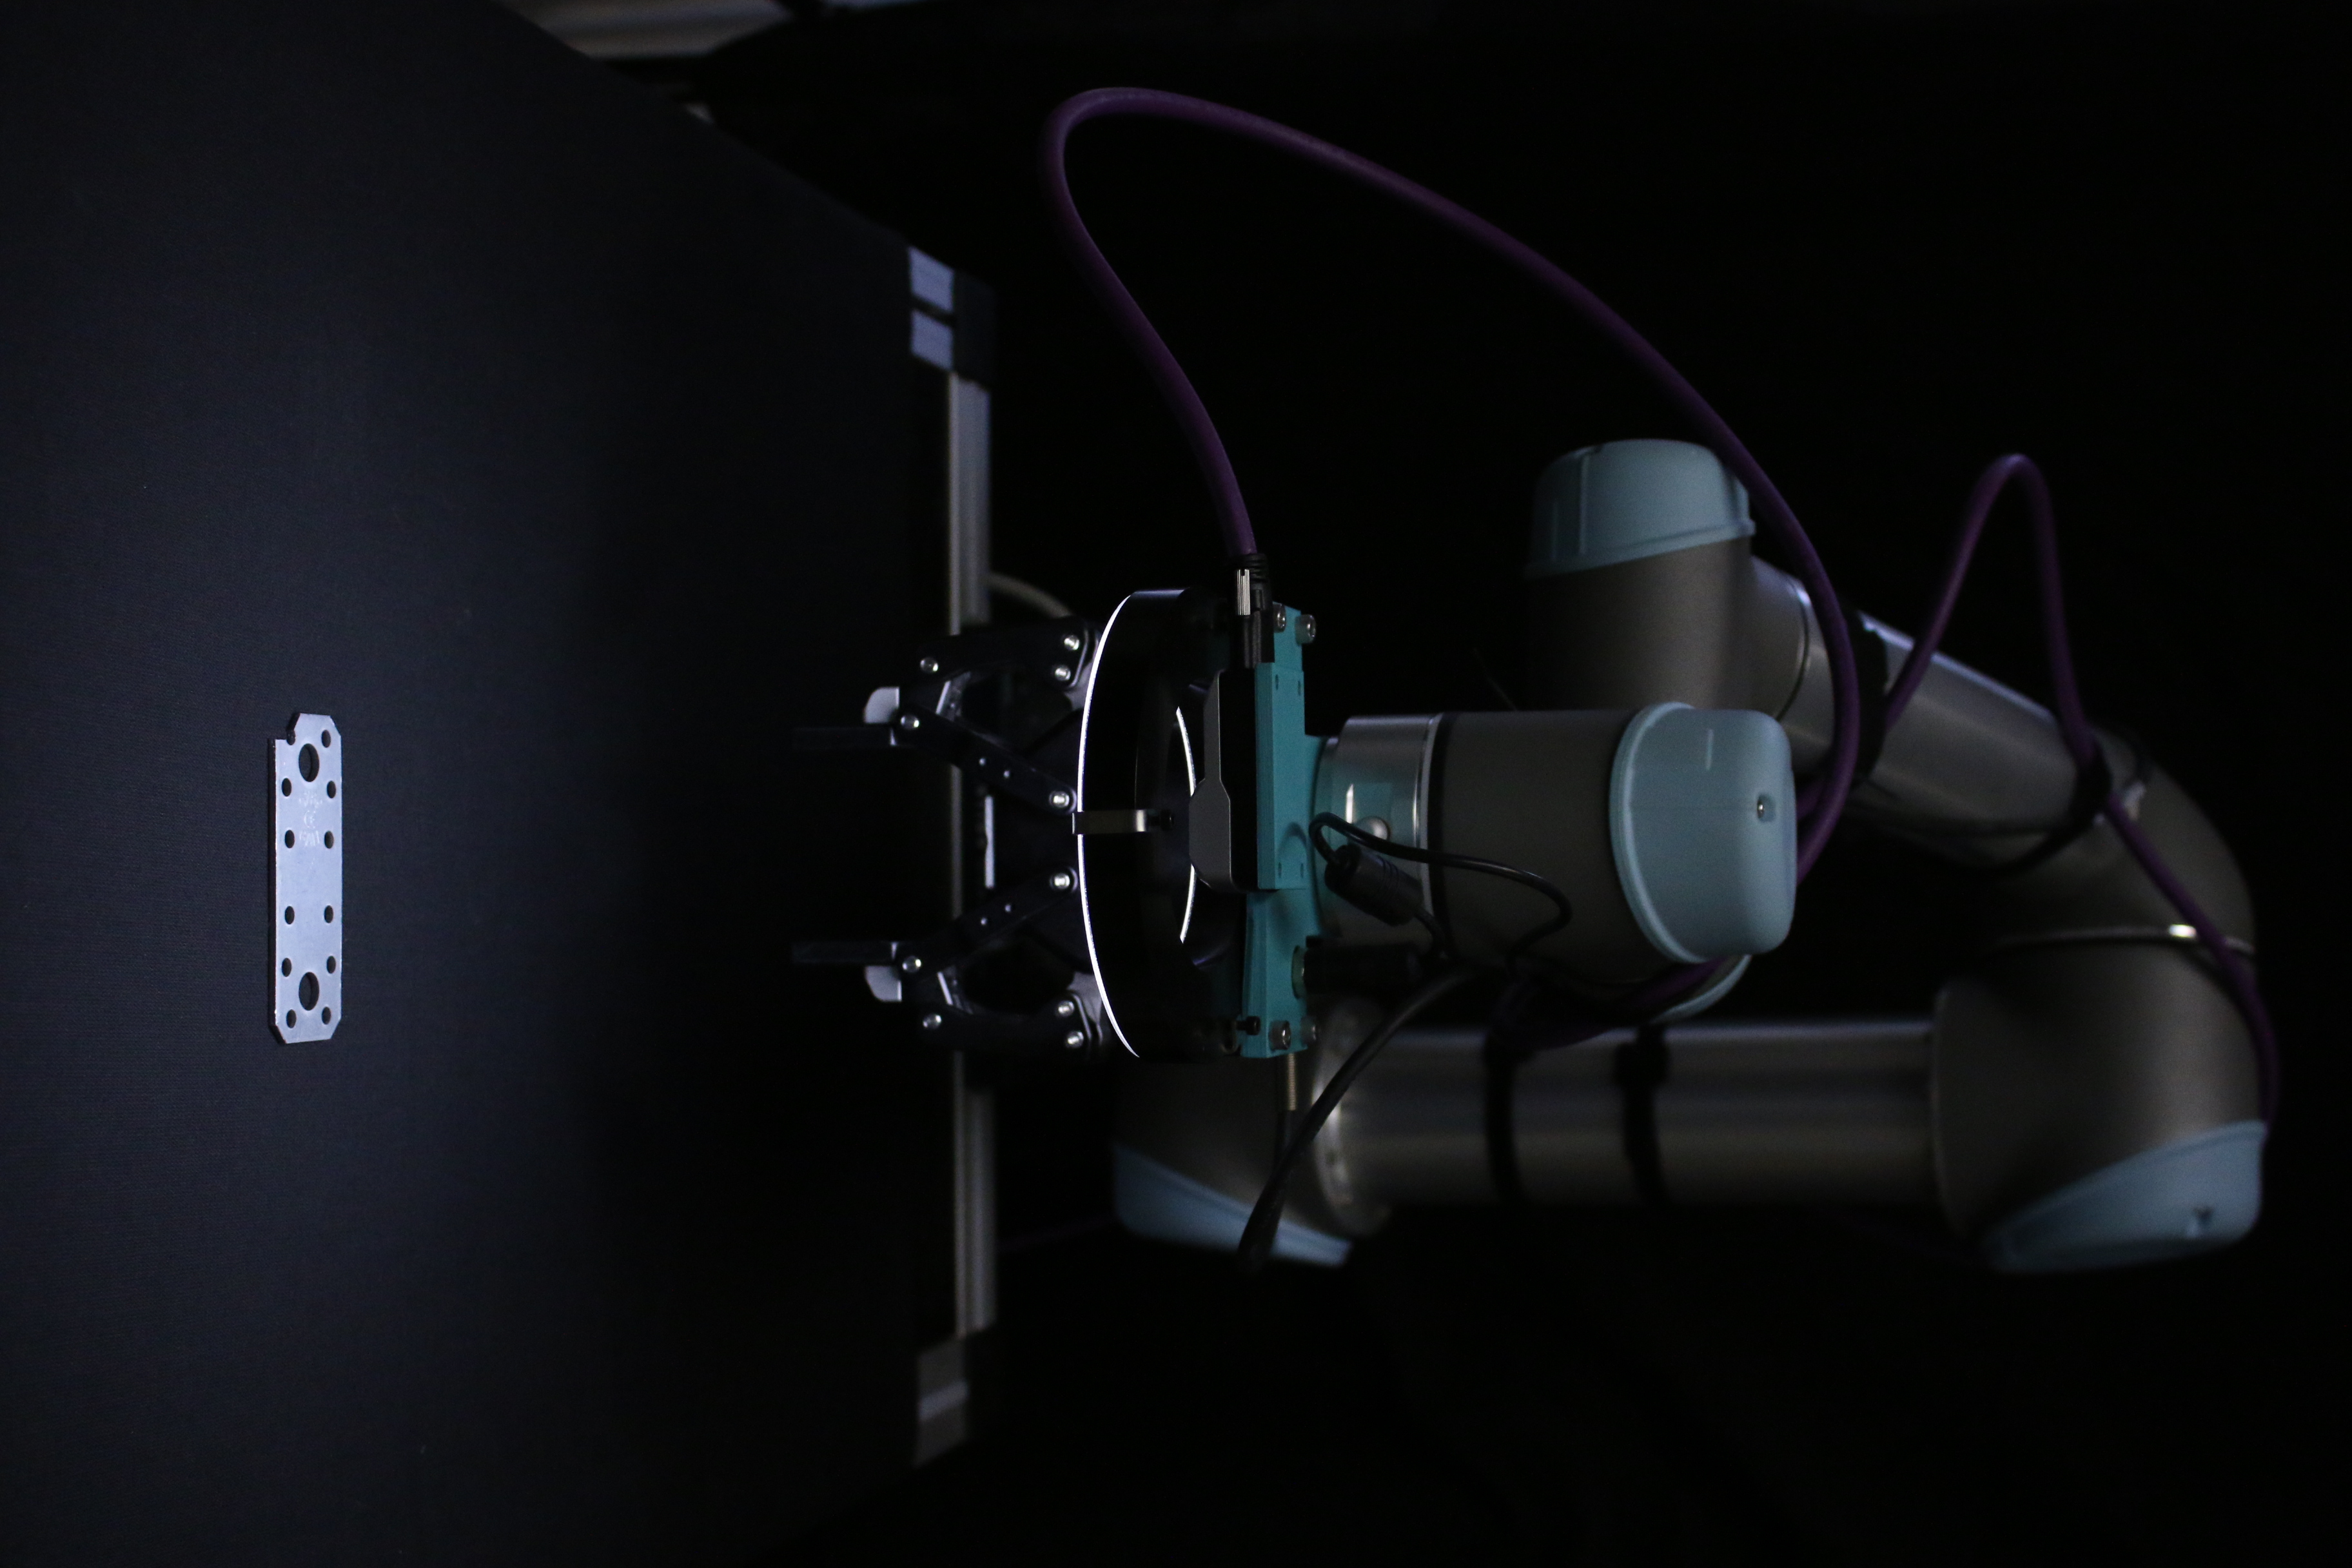
\includegraphics[angle=90, width=\textwidth]{figures/setupimages/setup_flachverbinder.JPG}
        %\caption*{Logical Anomalies}

    \end{subfigure}
    \begin{subfigure}[b]{0.3\textwidth}
        \centering
        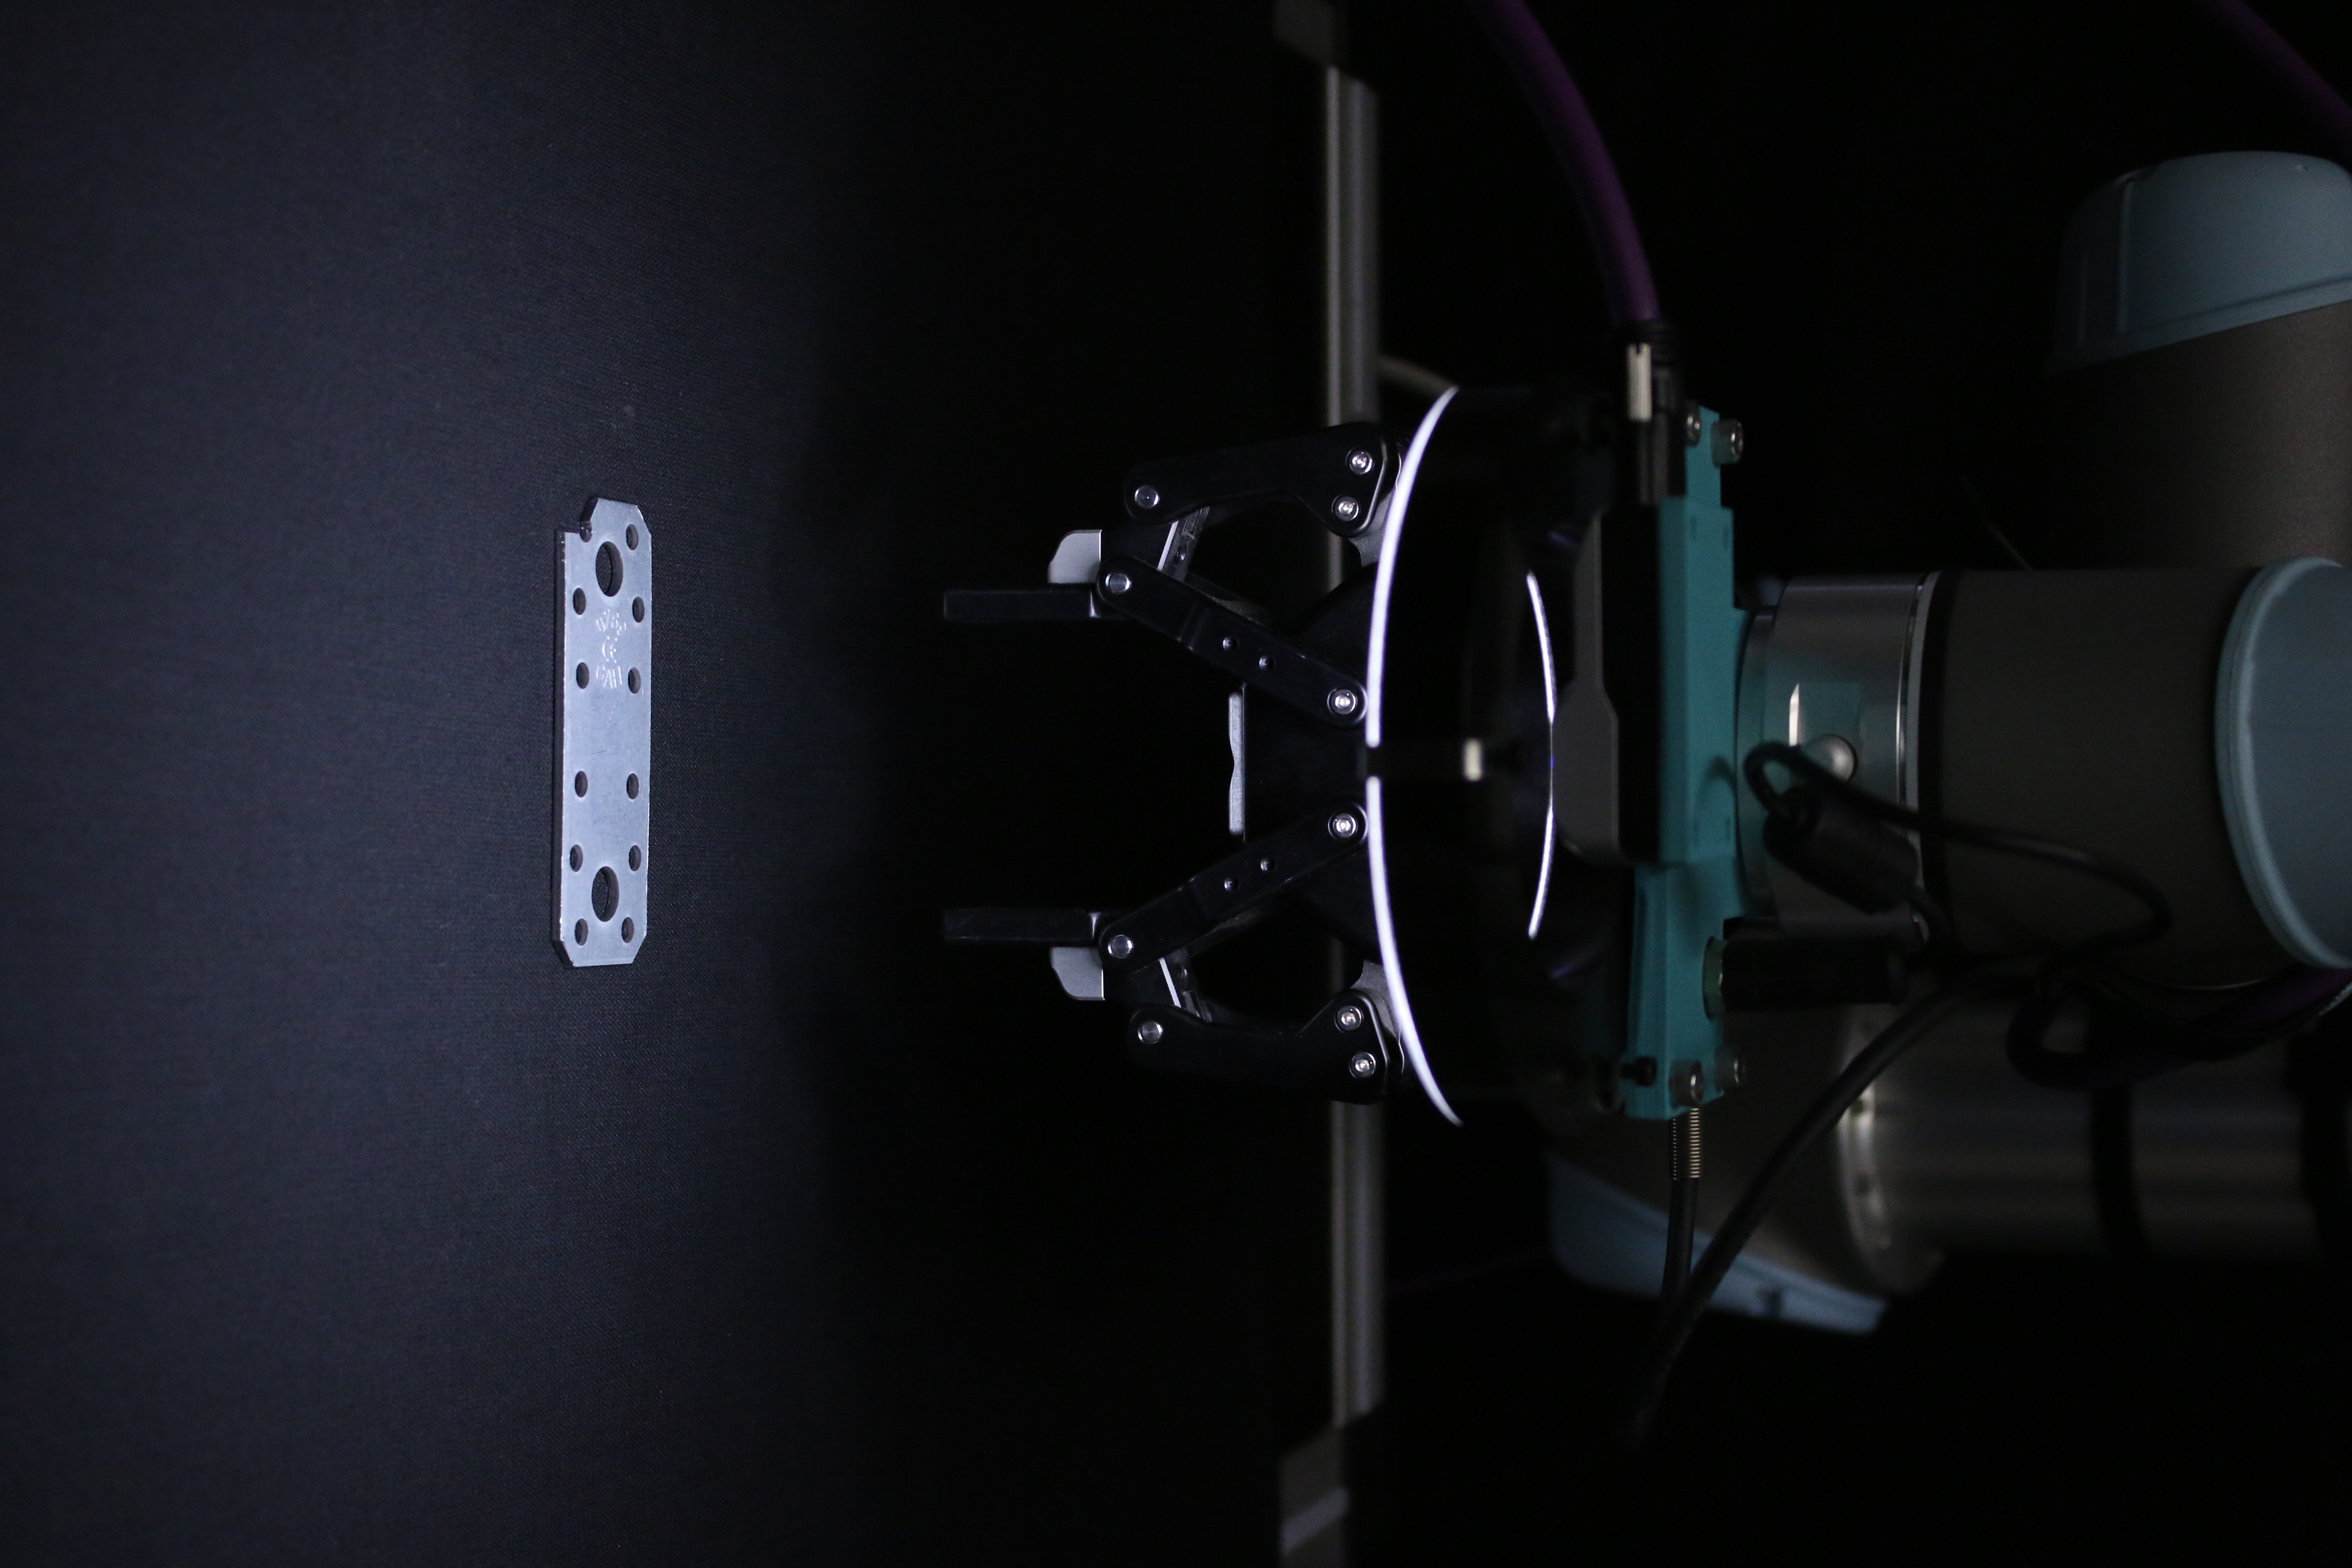
\includegraphics[angle=90, width=\textwidth]{figures/setupimages/setup_close.JPG}


    \end{subfigure}
    \caption{Images of the Environment of Data Collection}
    \label{fig:setupofdatacollection}
\end{figure}




\section{Anomalies}
\label{sec:flatconnectoranomalies}

To a certain degree the common MVTecAD LOCO clases all posess a balanced amount of logical and structural anomalies. Therefore the collection of possible anomalies for this class was kept at an even structural 
to logical ratio. The anomalies listed below can be viewed in figure xyz where exemplary anomalous images are displayed next to their corresponding ground truth mask.

\subsection{Structural Anomalies}
Structural anomalies in this case were comparably simple to think of an execute since they only involved damaging some area of the flat connector. Here we also tried to represent a variety of 
certain characteristics of anomalies among the ones we chose. An example would be to include anomalies with larger areays as well as ones with small ground truths.\newline
First of we produced the structural anomaly of a cut off corner. Ths was done by simply using a metal saw to remove a corner of the flat connector. This is an anomaly with a comparably large 
surface area and clean edges to predict. Next we again used a etal saw to damage the edges of the flat connector by cutting out pieces of or simply sawing into the edges of the object. One image 
of this anomaly type contained multiple damages spots on multiple edges. Due to the cuts partially being very small, this makes for an anomaly with very small ground truth areas as seen in figure 
xyz. As a last structural anomaly the saw was used to apply deep scratches on the object. This is mimicing another type of anomaly sometimes found in the classes of splicing connectors and pushpins 
in the original dataset. The common characteristic is that the region is very slim and long, making for better comparisons.

\subsection{Logical Anomalies}
The logical anomalies comprise the more interesting part of the anomaly types, as they are the focus of the MVTecAD LCOO dataset. The first logical anomaly in this class is the case in which a hole 
is missing in the flat connector hole pattern. This anomaly had to be improvised, since it is difficult to obtain a properly manufactured flat connector that was misproduced. To still include 
this type of anomaly, the solution was to first fill the hole with moldable material and then spray paint over it to hide color differences. For realism the spray paint color was the same as the 
object surface and the whole object was spray painted to avoid color artifacts. Partialy this anomaly was one of the larger and more clean cut ones since the holes mostly chosen to be filled were one of the two 
bigger ones on the object. For increased variety there were also anomlaous cases added where a small hole would be concealed. As a second anomaly the case of an extra hole was realised. To produce such an anomaly the facilities offered a drill, which was used to drill another small hole into 
the object at an unusual location. The size of the additional hole was the same as the smaller ones on the object. To also test capabilities of detecting multiple anomalies in a single image, this anomaly 
was put together with an differently sized hole. The final anomaly to be intruduced was a differently sized hole at a correct 
location. This would mean that the anomaly does not consist of the hole location but rather the size difference between this holes and the other ones in similar places. For this type of anomaly it 
is admissible to predict the whole hole as an anomalous region.  %vor der abgabe maybe die labels dafür noch anpassen dass es ringe sind
Here a drill tip was used with a slightly higher radius that the original hole to enlarge the diameter.


\subsection{Saturation Thresholds and Outlook}

The saturation scores for the anomalies, as discussed in section \ref{sec:datasets} were put at the amount of pixels in the anomalous region for all above listed anomalies respectively.
This was because the nature of presented anomalies of this categories calls for a full segmentation of the respective anomaly for a perfect result. Unlike in the pushpin example given in that section 
there are no cases that warrant multiple possible placements of anomalies.






